%======================================================================
\chapter{Implementation}
\label{ch: Chapter5}
%======================================================================
This chapter discusses the implementaion method setups and results for the three control algorithms.  The implementation methods are USB, raspberry pi, and mobile device.
%======================================================================
\section{Experimental Setup}
%----------------------------------------------------------------------
Before implementation was started setup needed to be done to get the system ready for testing.
%----------------------------------------------------------------------
\subsection{USB}
%----------------------------------------------------------------------
To setup for USB implementation the QFLEX 2 USB panel had to be installed onto the Quanser Aero.  Figure~\ref{fig:USB_Panel} is the USB panel.  Section~\ref{sec:USBtut} is a tutorial for the USB communication.
%----------------------------------------------------------------------
\subsection{Raspberry Pi}
%----------------------------------------------------------------------
Section~\ref{sec:RPItut} is the tutorial to setup and implement wireless communication using the raspberry pi.  The part that allows this implementation to be used is the QFLEX 2 EMBEDDED which is shown in figure~\ref{fig:Embedded_Panel}.  The communication protocol utilized by the Q-Flex2 embedded panel is SPI.  To enable this communication figure~\ref{fig:SPI_COM} is used in simulink.
\begin{figure}[!htbp]
    \centering
    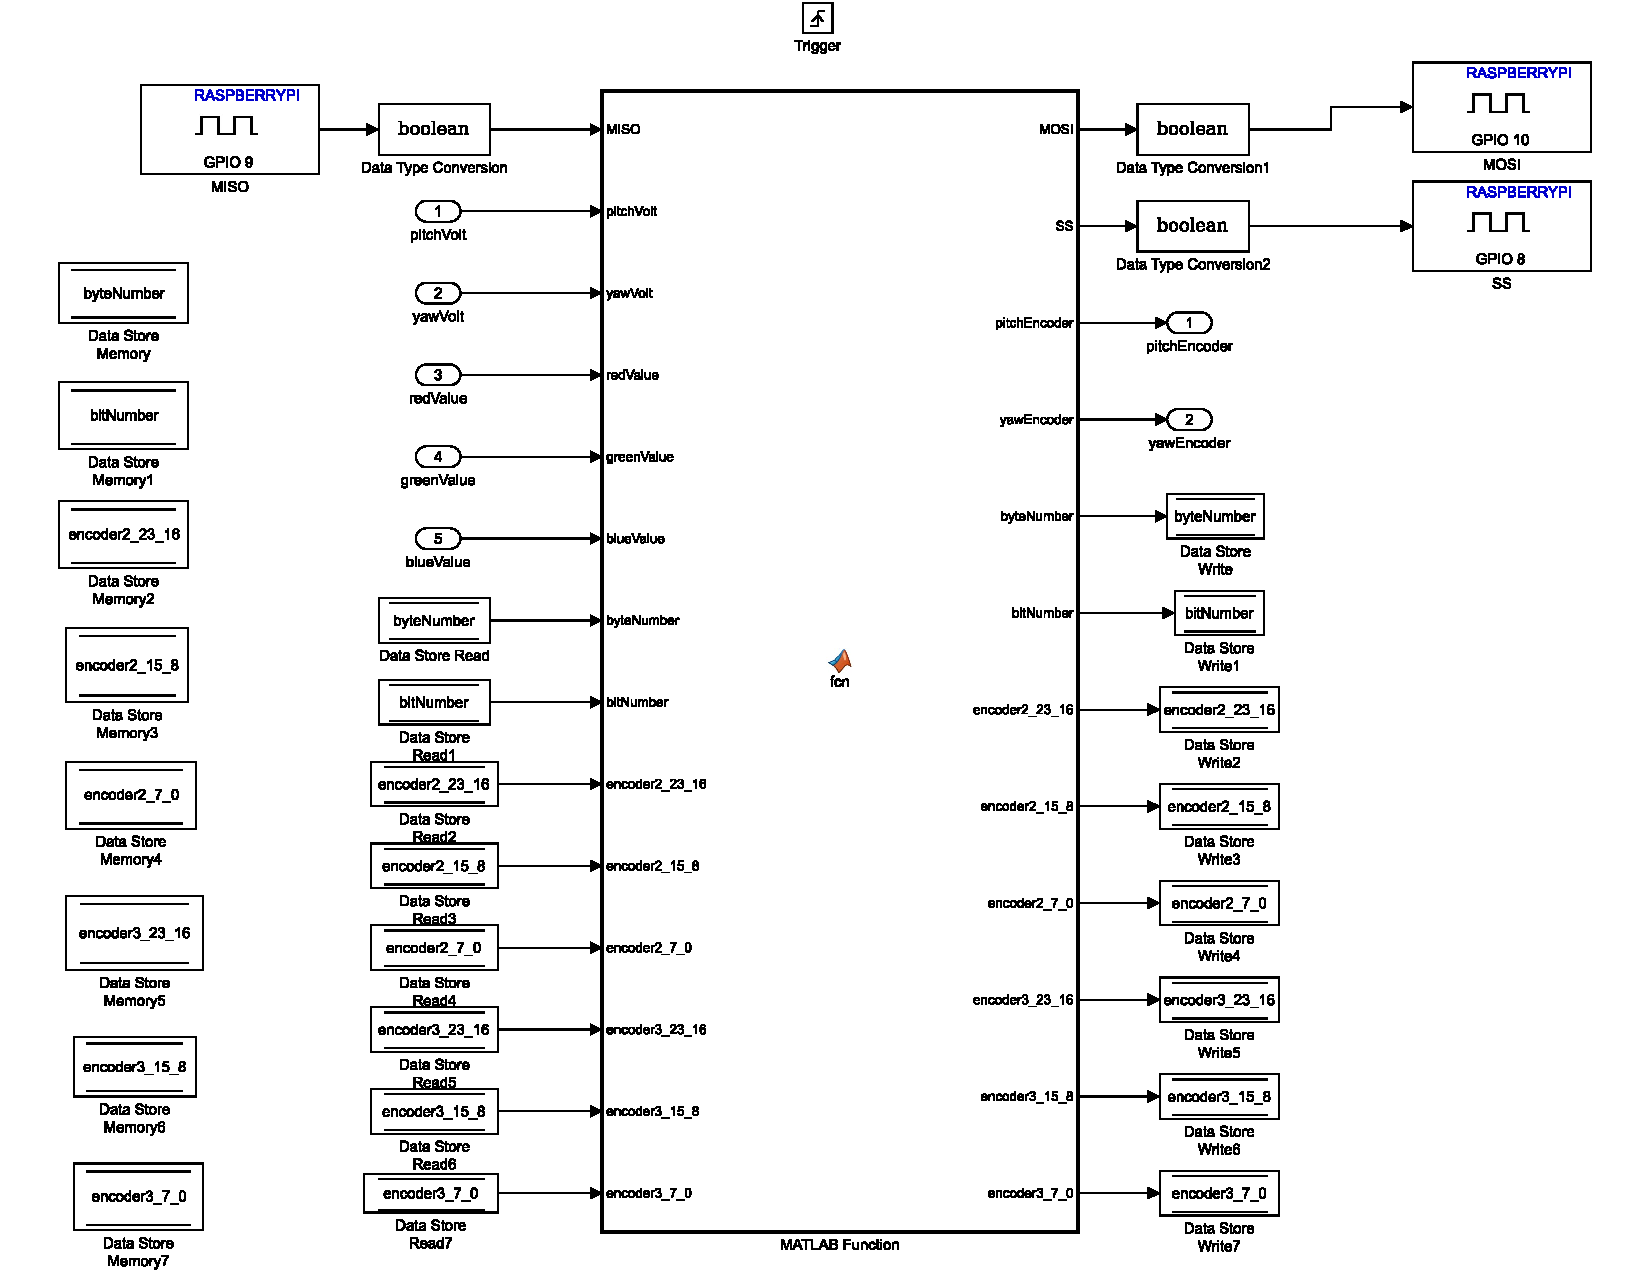
\includegraphics[width=.46\textwidth,keepaspectratio=true]{figs/img/SPI_COM.pdf}
    \caption{Block diagram of SPI communication protocol used for communication between the Raspberry Pi and Quanser Aero.}
    \label{fig:SPI_COM}
\end{figure}
%----------------------------------------------------------------------
\subsection{Mobile Device}
%----------------------------------------------------------------------
Section~\ref{sec:Androidtut} is the tutorial to setup and implement a simulink model using a mobile device as a user interface.  Figure~\ref{fig:Setup} is the physical lab setup for the mobile device experiment using two helicopters and two raspberry pi's. 
\begin{figure}[!htbp]
    \centering
    \includegraphics[width=.5\textwidth,keepaspectratio=true]{figs/ipe/Setup.eps}
    \caption{Experiment setup for controlling the Quanser Aeros via a mobile device.}
    \label{fig:Setup}
\end{figure}
Figure~\ref{fig:TCPModel} is the TCP communication model between the mobile device and the raspberry pi.
%\todo[inline]{Ken needs to describe figure~\ref{fig:TCPModel} more}
When a user wants to send a configuration to the helicopter, the mobile device's network interface card recognizes the protocol that is being used.  In this case, UDP is used to maximize the transmission speed.  Metadata is appended to the orginal data for routing purposes.  After the packet is prepared, it is sent to the wirless router and across the network.  Once it reaches the raspberry pi, it discards the metadata and uses the remaining data to calculate the voltage to apply to the helicopter.
\begin{figure}[!htbp]
    \centering
    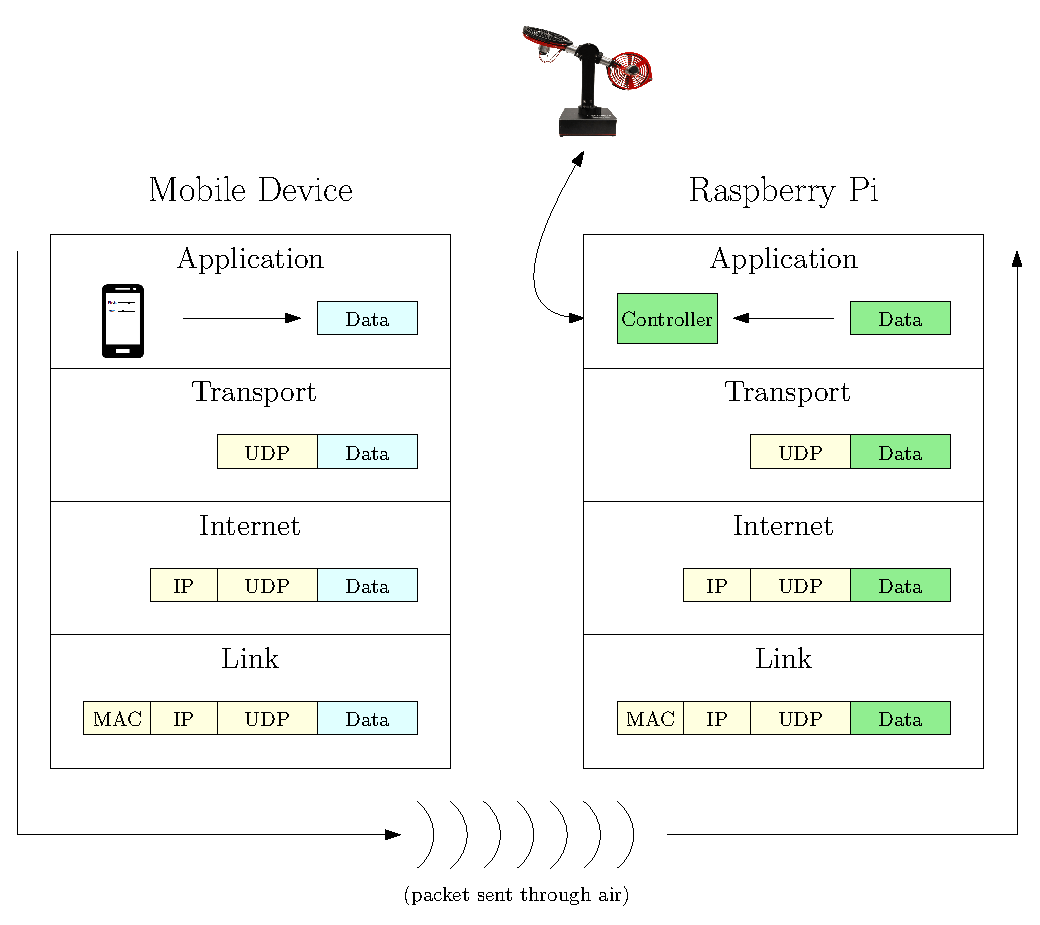
\includegraphics[width=.46\textwidth,keepaspectratio=true]{figs/ipe/TCPModel.eps}
    \caption{Illustration of the TCP model which describes how packets are sent and recieved from mobile devices to the Quanser Aero.}
    \label{fig:TCPModel}
\end{figure}
Figure~\ref{fig:Android_Interface} is the simulink model to generate the mobile device application.
\begin{figure}[!htbp]
    \centering
    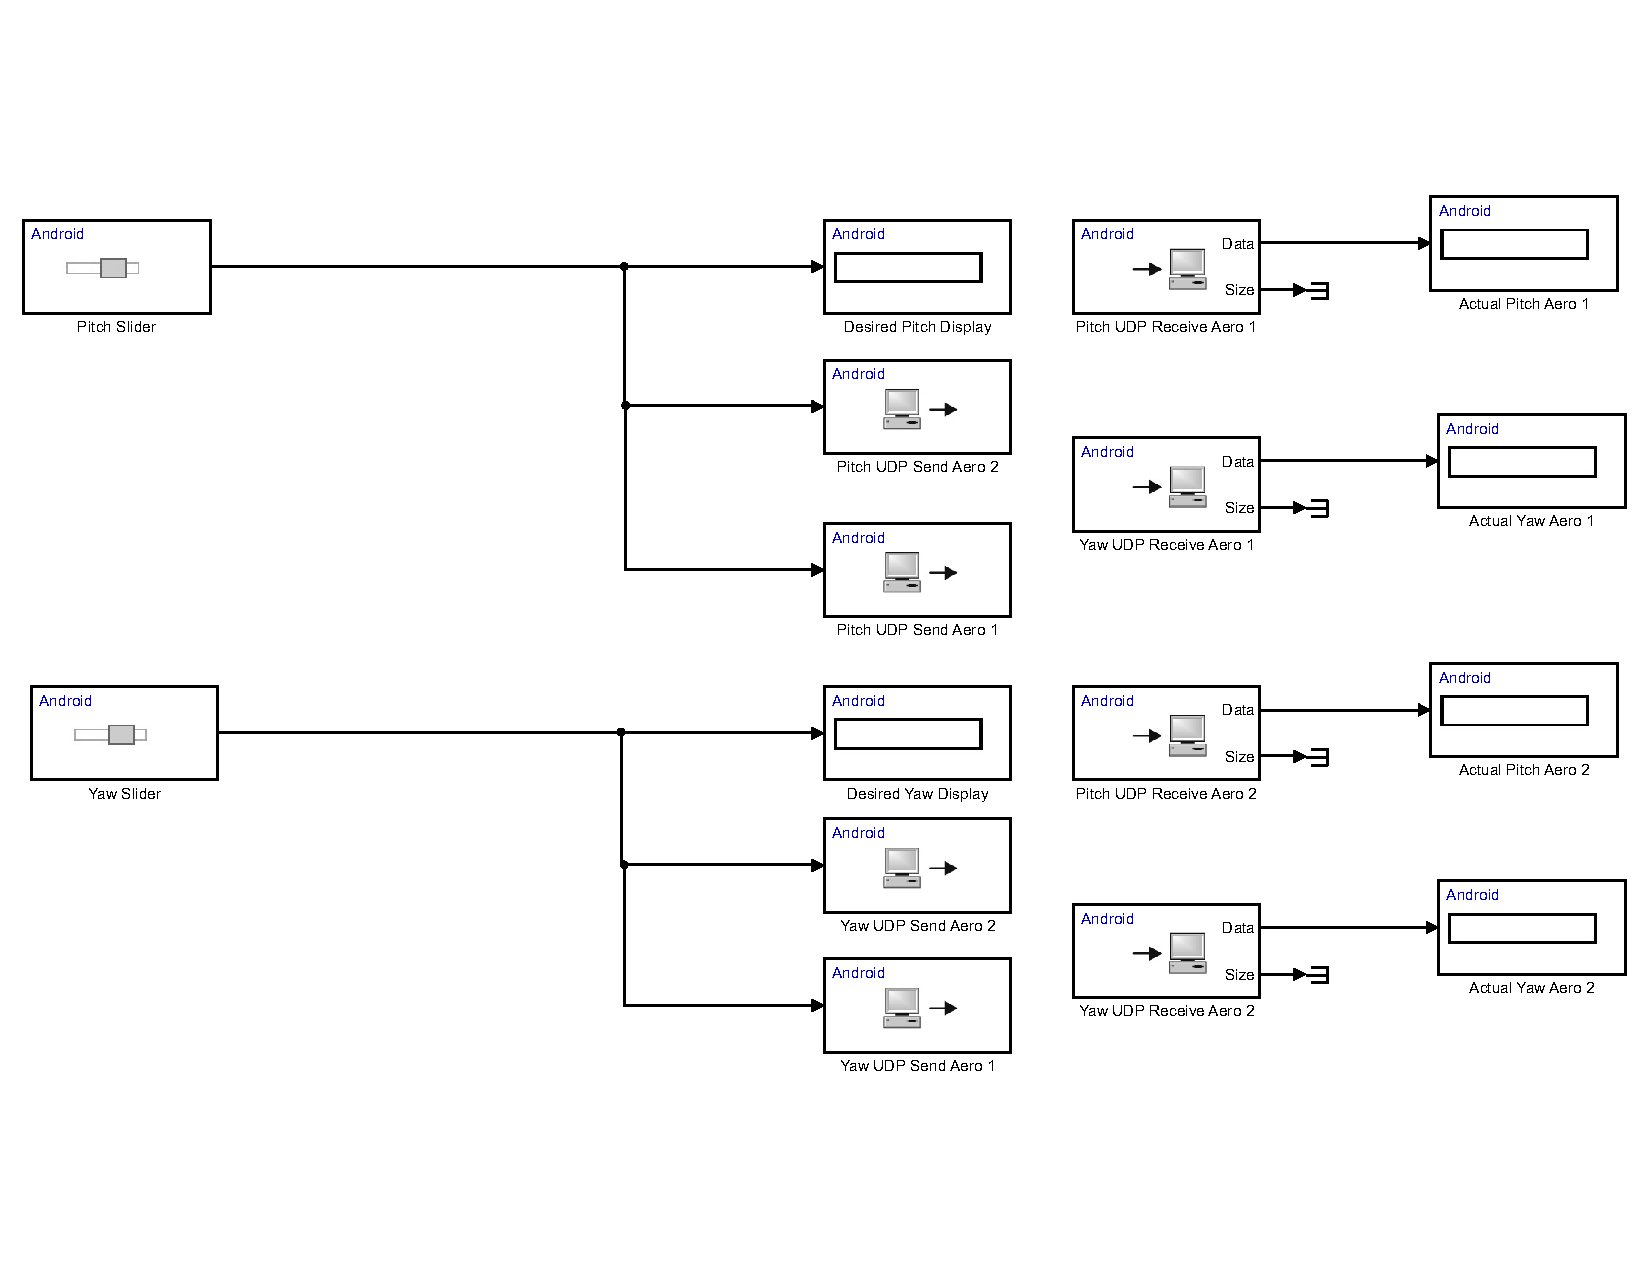
\includegraphics[width=.46\textwidth,keepaspectratio=true]{figs/img/Android_Interface_2Aero}
    \caption{Simulink model of the android interface using two Quanser Aeros.}
    \label{fig:Android_Interface}
\end{figure}
A screenshot of the application is shown in figure~\ref{fig:Screenshot_Android_Interface}.  As it can be seen, the application displays the actual pitch and yaw configurations for both helicopters.  It also displays the desired configuration that is being set by the two slide bars.
\begin{figure}[!htbp]
    \centering
    \includegraphics[width=.46\textwidth,keepaspectratio=true]{figs/img/Screenshot_Android_Interface_2Aero}
    \caption{Screenshot of the mobile user interface.}
    \label{fig:Screenshot_Android_Interface}
\end{figure}

%======================================================================
\section{USB}
%----------------------------------------------------------------------
Before we tested using wireless communication the algorithms had to be tested using a wired connection to make sure they worked properly.  This connection was done using a USB cable and the QFLEX 2 USB panel.  Over the next couple of sections the experiment on the Quanser Aero using the USB connection is discussed.
%----------------------------------------------------------------------
\subsection{LQR}
%----------------------------------------------------------------------
For the LQR motion control algoritm, two types of controllers were implemented.  These are P type and PI type controllers.  Figure~\ref{fig:LQR_P_USB_Block_Diagram} is the simulink model for the LQR P type controller using the USB connection to the PC.  In the model the desired input configurations are taken in and applied to the LQR P type controller, which calculates the voltages to be applied to the motors of the helicopter.  These voltages are applied directly to the helicopter using the USB connection.
\begin{figure}[!htbp]
    \centering
    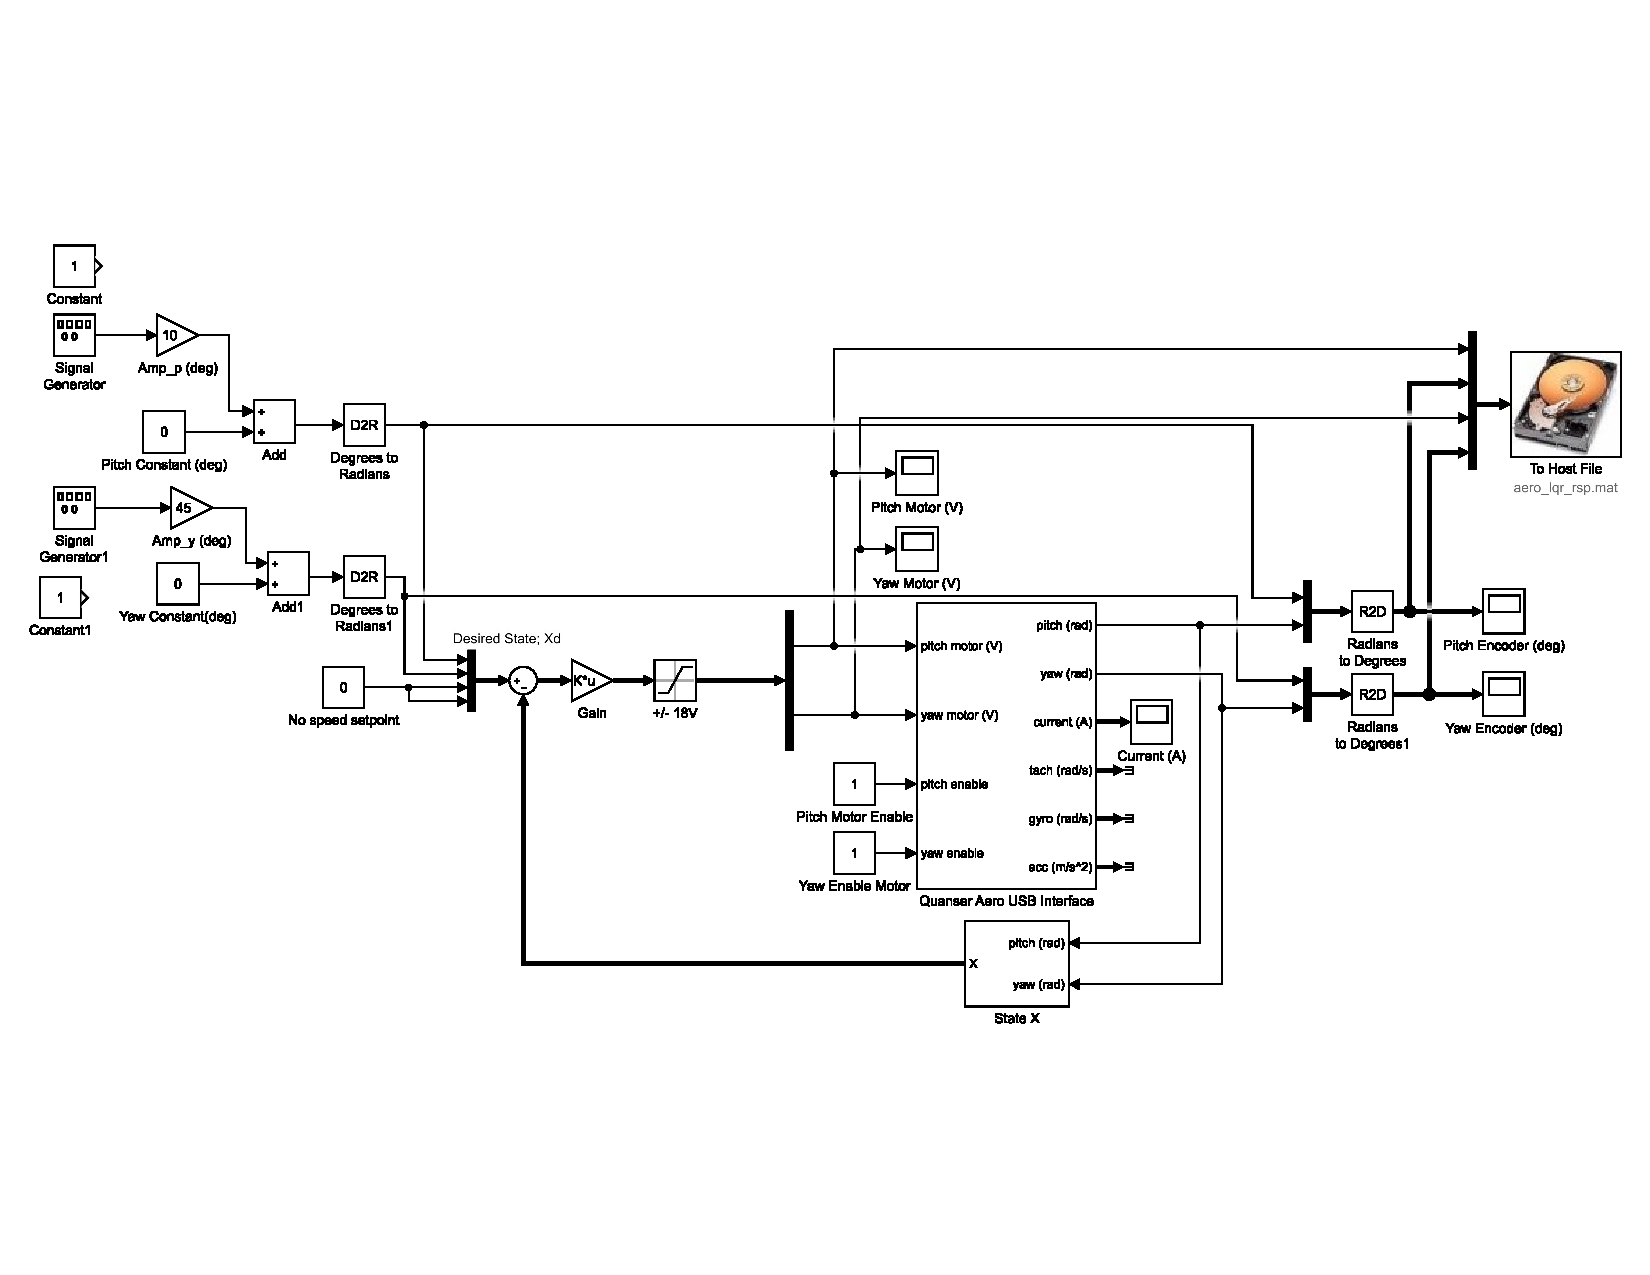
\includegraphics[width=.8\textwidth,keepaspectratio=true]{figs/img/LQR_USB}
    \caption{Block diagram for LQR P type controller with a USB connection.}
    \label{fig:LQR_P_USB_Block_Diagram}
\end{figure}
%\todo[inline]{Insert LQR PI Block Diagram}

Figure~\ref{fig:LQR_PI_USB_Block_Diagram} is the simulink model for the LQR PI type controller using the USB connection.  In the model the desired input configurations are taken in and applied to the LQR PI type controller, which calculates the voltages to be applied to the motors of the helicopter.  These voltages are applied directly to the helicopter using the USB connection.
\begin{figure}[!htbp]
    \centering
    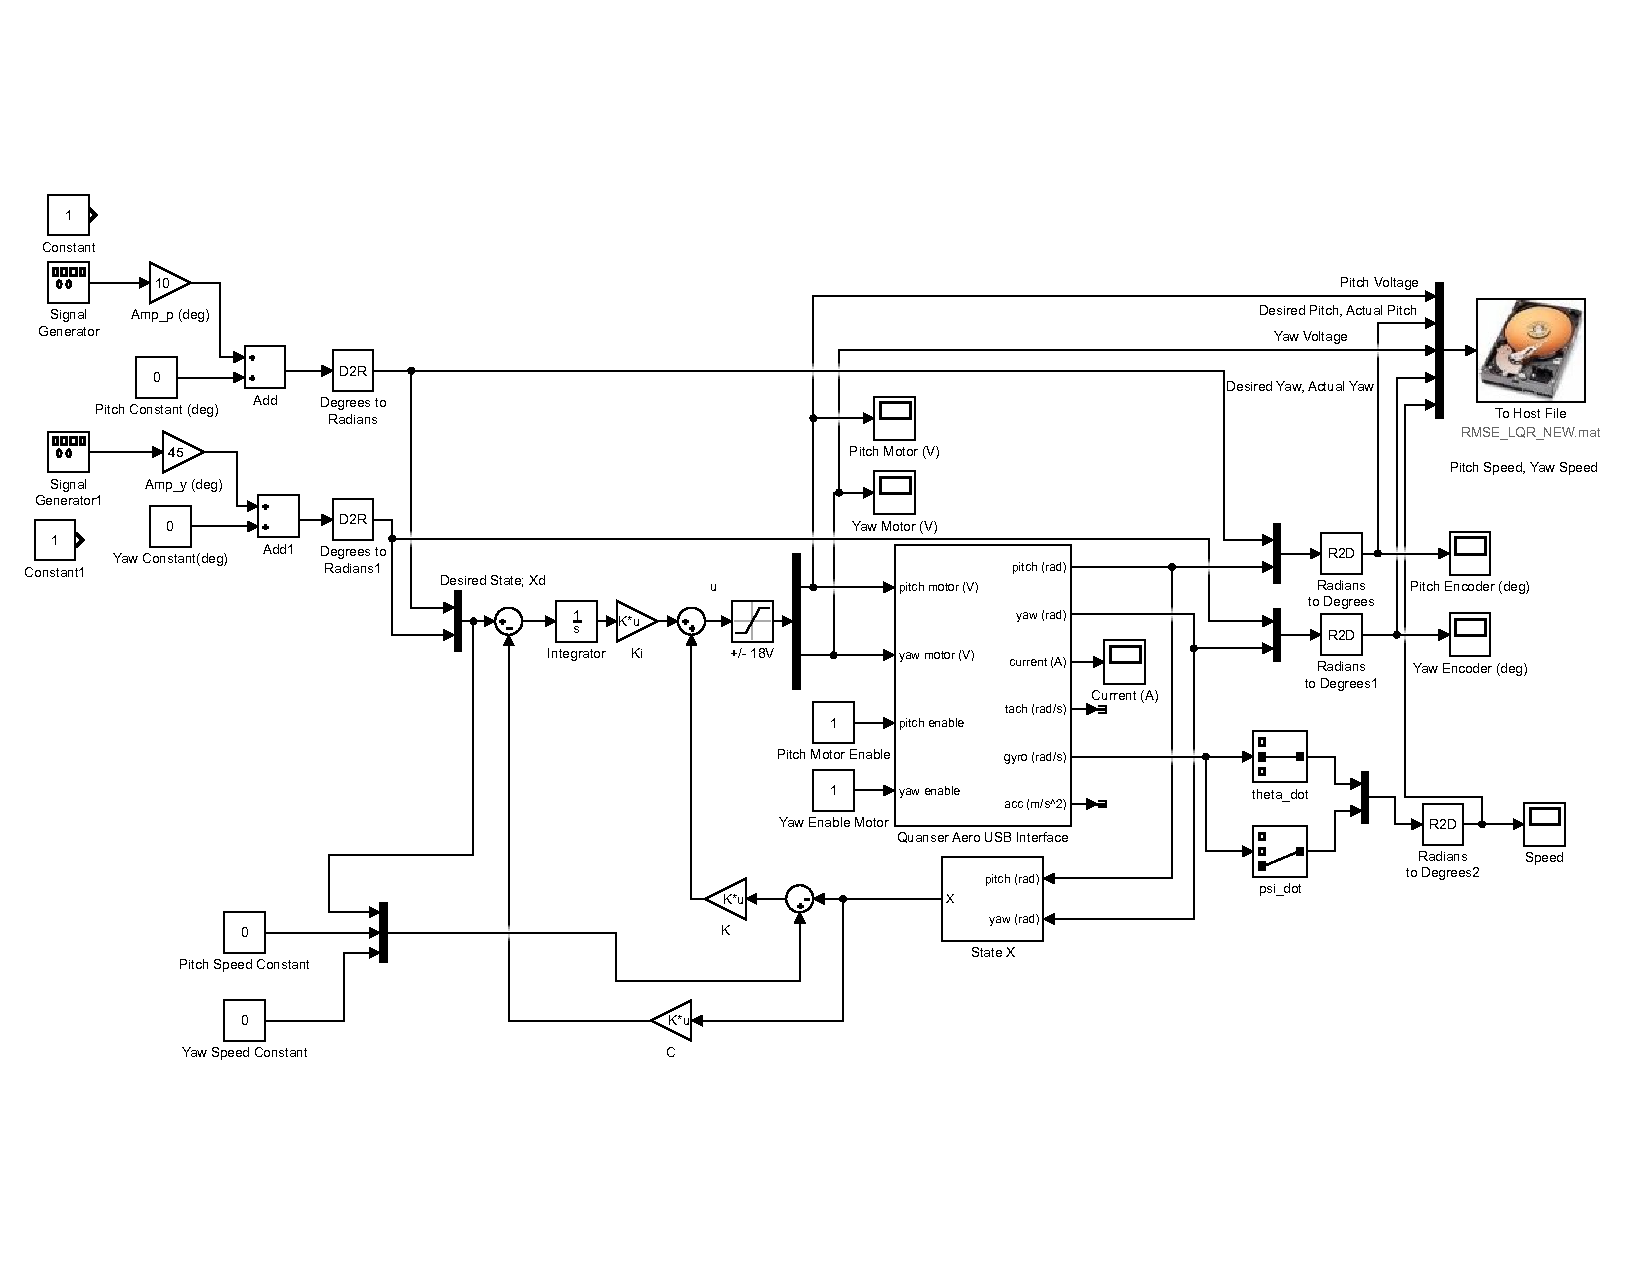
\includegraphics[width=.8\textwidth,keepaspectratio=true]{figs/img/LQR_PI_USB}
    \caption{Block diagram for LQR PI type controller with a USB connection.}
    \label{fig:LQR_PI_USB_Block_Diagram}
\end{figure}

Figure~\ref{fig:PvsPI_Step} shows the wave forms for a step input while comparing LQR P type to LQR PI type controllers.  Figure~\ref{fig:Pitch_LQR_RMSE_Step} shows the pitch values of the controllers and the desired.  Figure~\ref{fig:Yaw_LQR_RMSE_Step} shows the yaw values of the controllers and the desired.  Figure~\ref{fig:PitchVoltage_LQR_RMSE_Step} shows the voltages being applied to the main motor for both controllers.  Figure~\ref{fig:YawVoltage_LQR_RMSE_Step} shows the voltages being applied to the tail motor for both controllers.  Figure~\ref{fig:PitchSpeed_LQR_RMSE_Step} displays the speeds of the motion in the pitch direction for both controllers.  Figure~\ref{fig:YawSpeed_LQR_RMSE_Step} displays the speeds of the motion in the yaw direction for both controllers.
\begin{figure}[!htbp]
    \centering
    \subfigure[][]{
    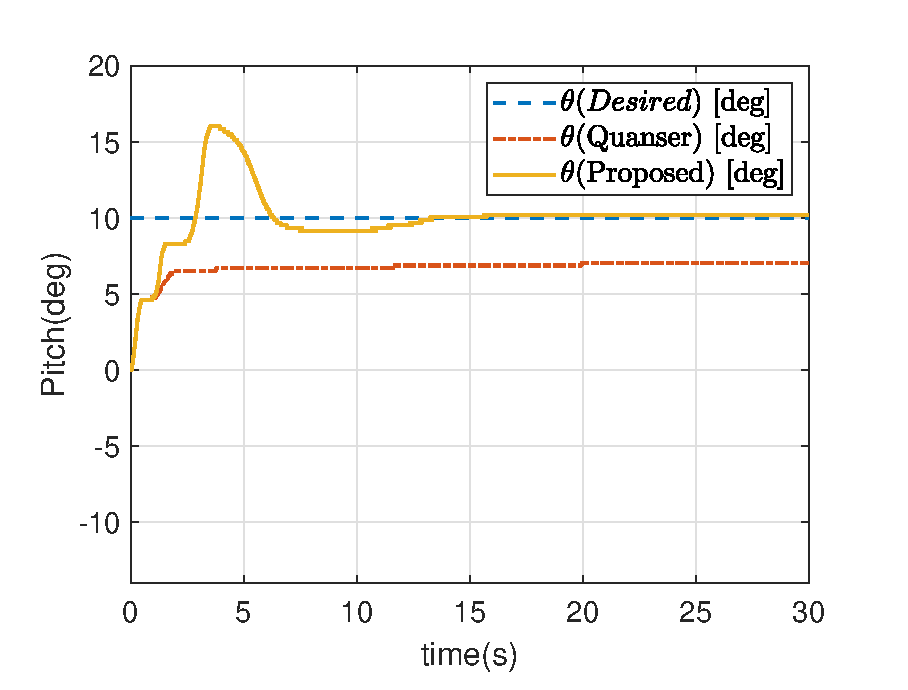
\includegraphics[width=.46\textwidth,keepaspectratio=true]{figs/matlab/LQR_PIvLQR_P_USB/step/Pitch_LQR_RMSE.eps}
    \label{fig:Pitch_LQR_RMSE_Step}
    }
    \subfigure[][]{
    \includegraphics[width=.46\textwidth,keepaspectratio=true]{figs/matlab/LQR_PIvLQR_P_USB/step/Yaw_LQR_RMSE.eps}
    \label{fig:Yaw_LQR_RMSE_Step}
    }    
    \subfigure[][]{
    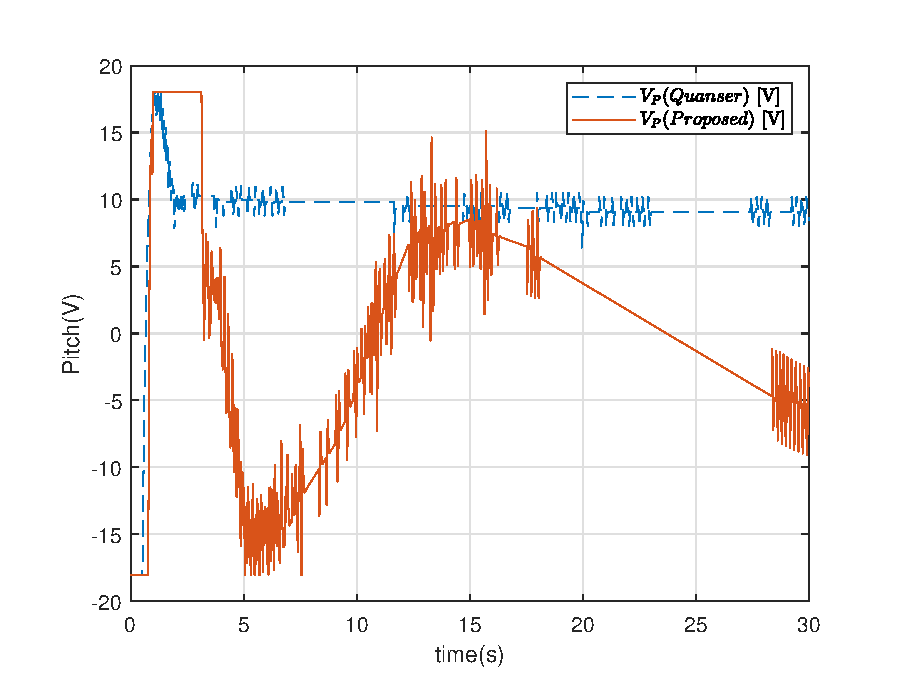
\includegraphics[width=.46\textwidth,keepaspectratio=true]{figs/matlab/LQR_PIvLQR_P_USB/step/PitchVoltage_LQR_RMSE.eps}
    \label{fig:PitchVoltage_LQR_RMSE_Step}
    }    
    \subfigure[][]{
    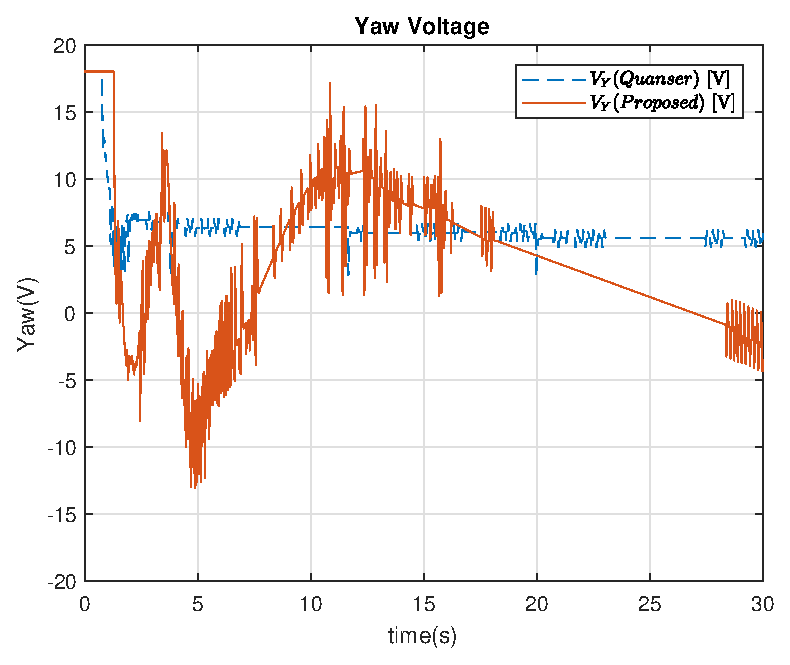
\includegraphics[width=.46\textwidth,keepaspectratio=true]{figs/matlab/LQR_PIvLQR_P_USB/step/YawVoltage_LQR_RMSE.eps}
    \label{fig:YawVoltage_LQR_RMSE_Step}
    }
    \subfigure[][]{
    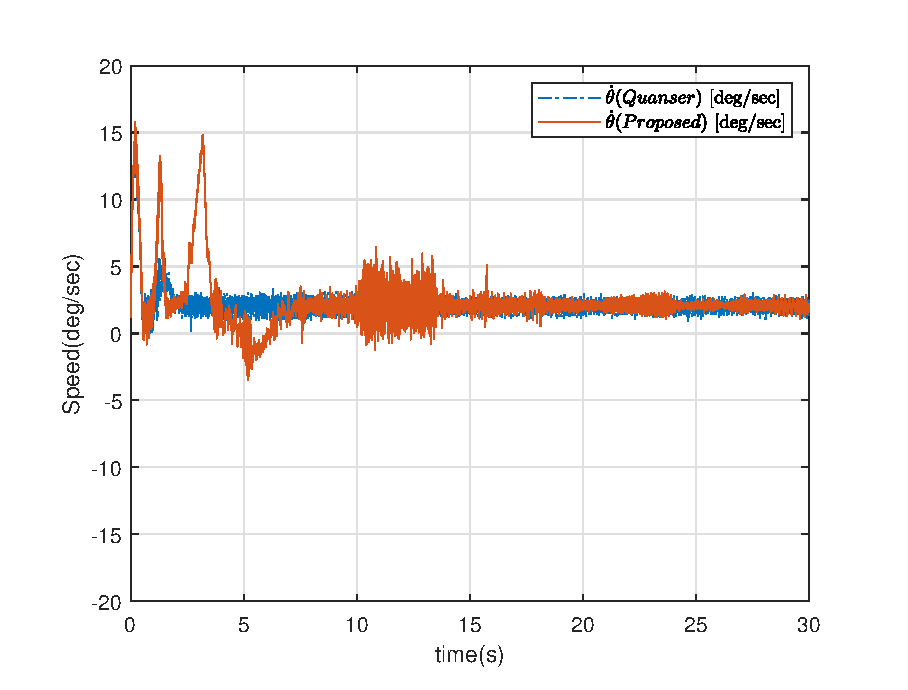
\includegraphics[width=.46\textwidth,keepaspectratio=true]{figs/matlab/LQR_PIvLQR_P_USB/step/PitchSpeed_LQR_RMSE.eps}
    \label{fig:PitchSpeed_LQR_RMSE_Step}
    }
    \subfigure[][]{
    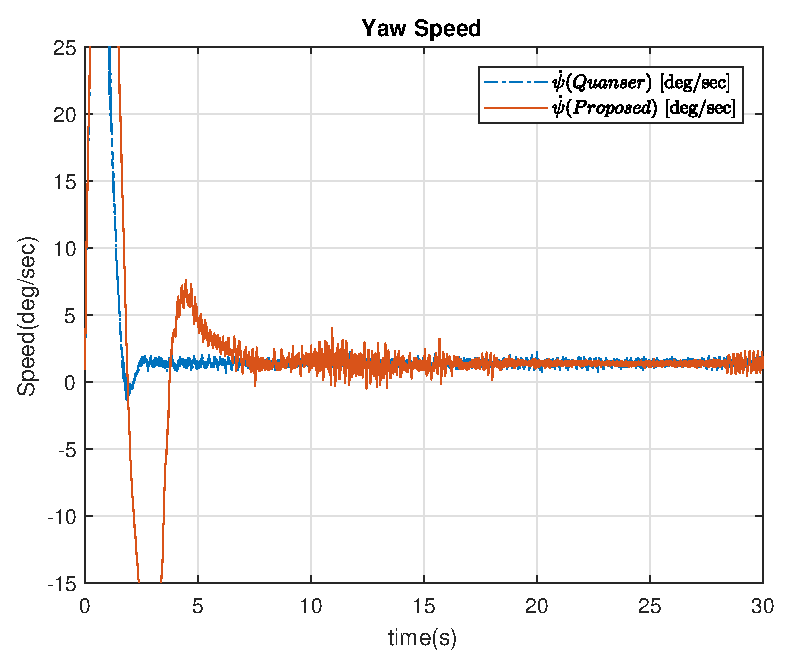
\includegraphics[width=.46\textwidth,keepaspectratio=true]{figs/matlab/LQR_PIvLQR_P_USB/step/YawSpeed_LQR_RMSE.eps}
    \label{fig:YawSpeed_LQR_RMSE_Step}
    }
    \caption{USB implementation for proportional controller and proportional-integral controller calculated by LQR with a step input.}
    \label{fig:PvsPI_Step}
\end{figure}
Figure~\ref{fig:PvsPI_Square} and figure~\ref{fig:PvsPI_Sine} have similar figures to figure~\ref{fig:PvsPI_Step}, except figure~\ref{fig:PvsPI_Square} has a square wave input and figure~\ref{fig:PvsPI_Sine} has a sine wave input.
\begin{figure}[!htbp]
    \centering
    \subfigure[][]{
    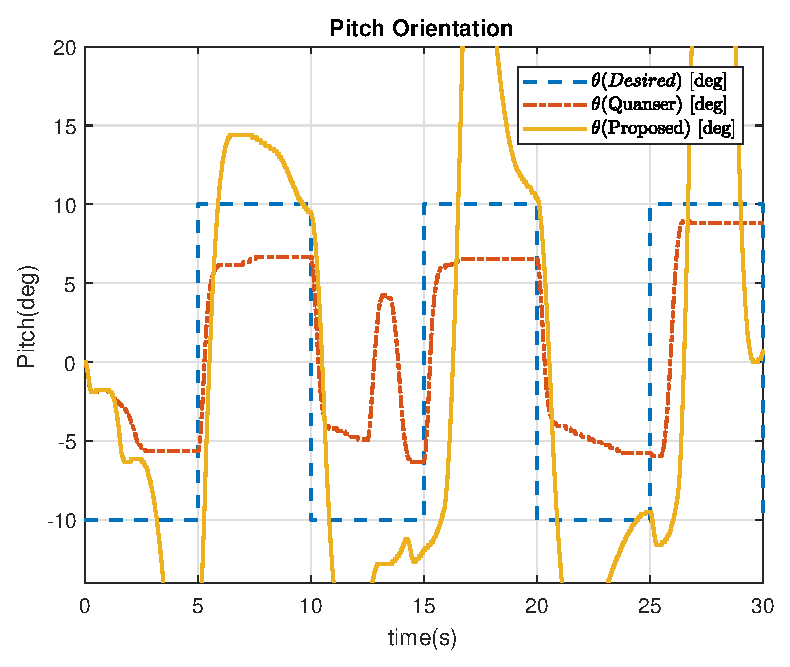
\includegraphics[width=.46\textwidth,keepaspectratio=true]{figs/matlab/LQR_PIvLQR_P_USB/square/Pitch_LQR_RMSE.eps}
    \label{fig:Pitch_LQR_RMSE_Square}
    }
    \subfigure[][]{
    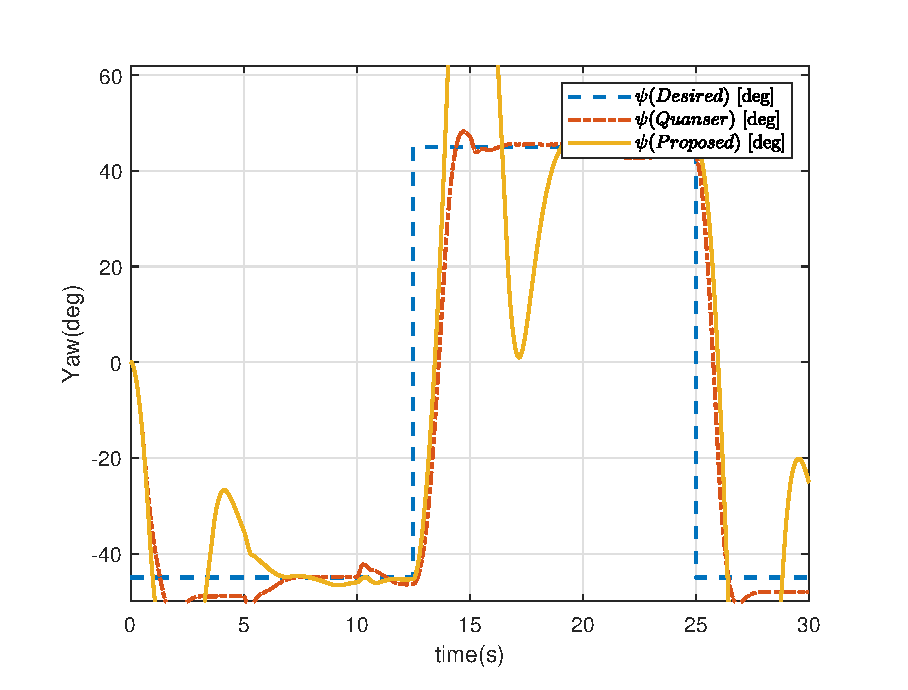
\includegraphics[width=.46\textwidth,keepaspectratio=true]{figs/matlab/LQR_PIvLQR_P_USB/square/Yaw_LQR_RMSE.eps}
    \label{fig:Yaw_LQR_RMSE_Square}
    }    
    \subfigure[][]{
    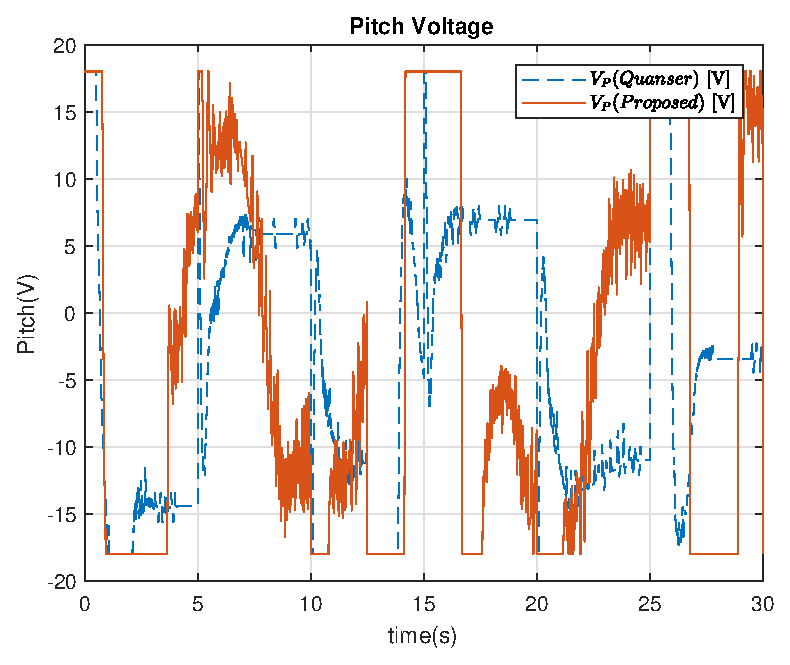
\includegraphics[width=.46\textwidth,keepaspectratio=true]{figs/matlab/LQR_PIvLQR_P_USB/square/PitchVoltage_LQR_RMSE.eps}
    \label{fig:PitchVoltage_LQR_RMSE_Square}
    }    
    \subfigure[][]{
    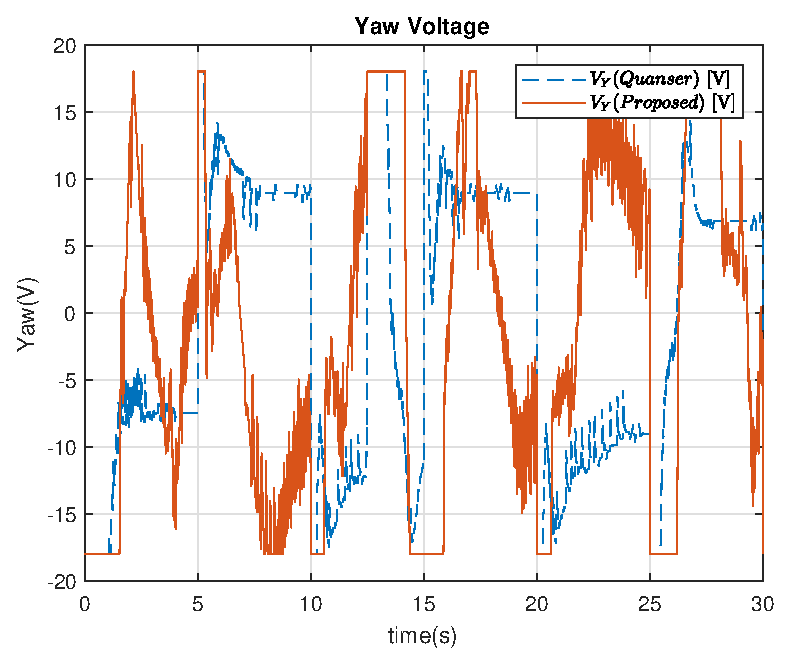
\includegraphics[width=.46\textwidth,keepaspectratio=true]{figs/matlab/LQR_PIvLQR_P_USB/square/YawVoltage_LQR_RMSE.eps}
    \label{fig:YawVoltage_LQR_RMSE_Square}
    }
    \subfigure[][]{
    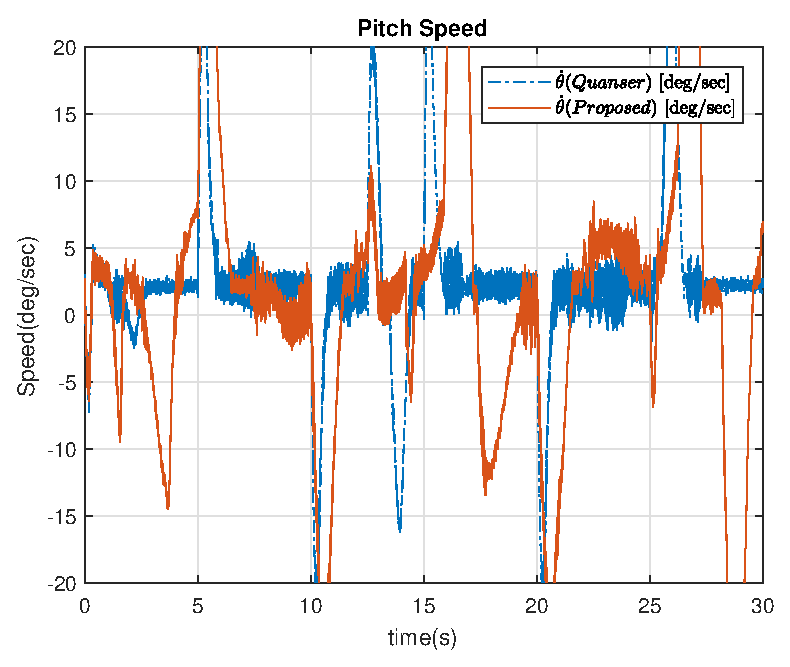
\includegraphics[width=.46\textwidth,keepaspectratio=true]{figs/matlab/LQR_PIvLQR_P_USB/square/PitchSpeed_LQR_RMSE.eps}
    \label{fig:PitchSpeed_LQR_RMSE_Square}
    }
    \subfigure[][]{
    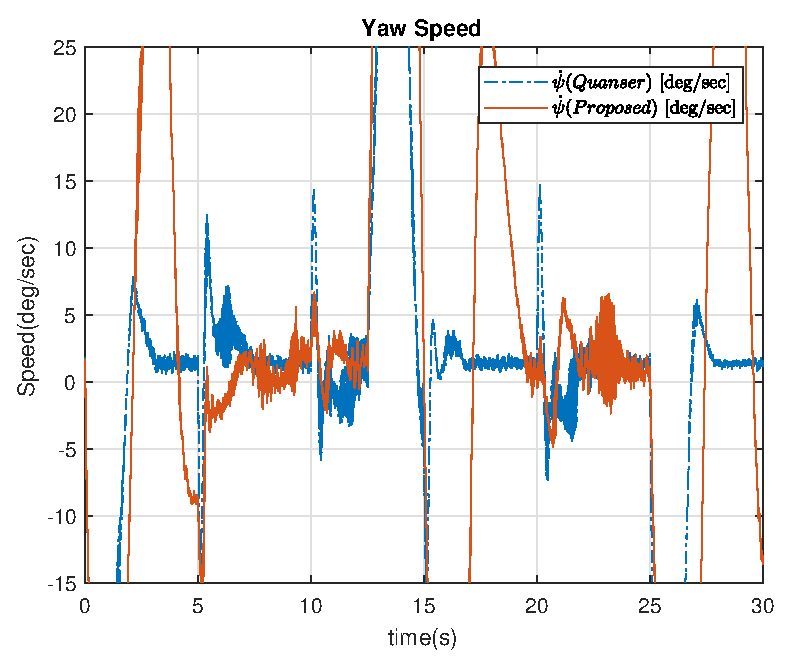
\includegraphics[width=.46\textwidth,keepaspectratio=true]{figs/matlab/LQR_PIvLQR_P_USB/square/YawSpeed_LQR_RMSE.eps}
    \label{fig:PitchSpeed_LQR_RMSE_Square}
    }
    \caption{USB implementation for proportional controller and proportional-integral controller calculated by LQR with a square wave input.}
    \label{fig:PvsPI_Square}
\end{figure}

\begin{figure}[!htbp]
    \centering
    \subfigure[][]{
    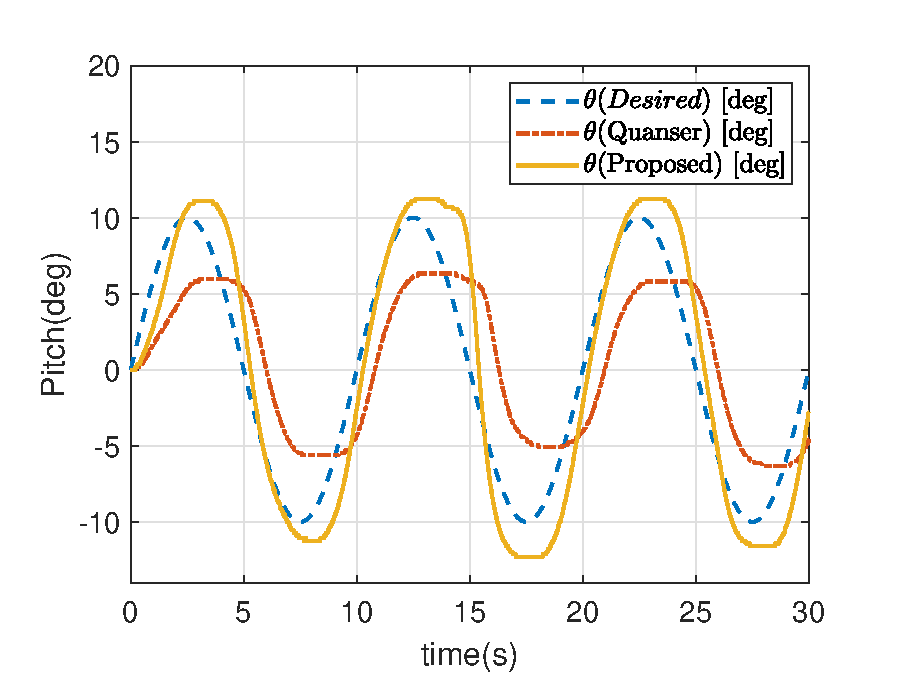
\includegraphics[width=.46\textwidth,keepaspectratio=true]{figs/matlab/LQR_PIvLQR_P_USB/sine/Pitch_LQR_RMSE.eps}
    \label{fig:Pitch_LQR_RMSE_Sine}
    }
    \subfigure[][]{
    \includegraphics[width=.46\textwidth,keepaspectratio=true]{figs/matlab/LQR_PIvLQR_P_USB/sine/Yaw_LQR_RMSE.eps}
    \label{fig:Yaw_LQR_RMSE_Sine}
    }    
    \subfigure[][]{
    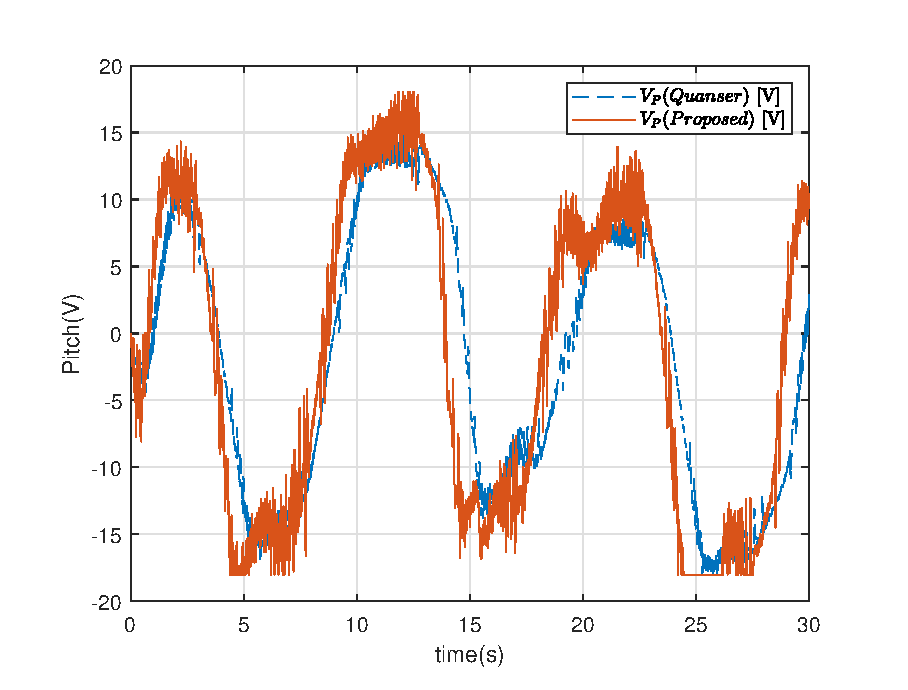
\includegraphics[width=.46\textwidth,keepaspectratio=true]{figs/matlab/LQR_PIvLQR_P_USB/sine/PitchVoltage_LQR_RMSE.eps}
    \label{fig:PitchVoltage_LQR_RMSE_Sine}
    }    
    \subfigure[][]{
    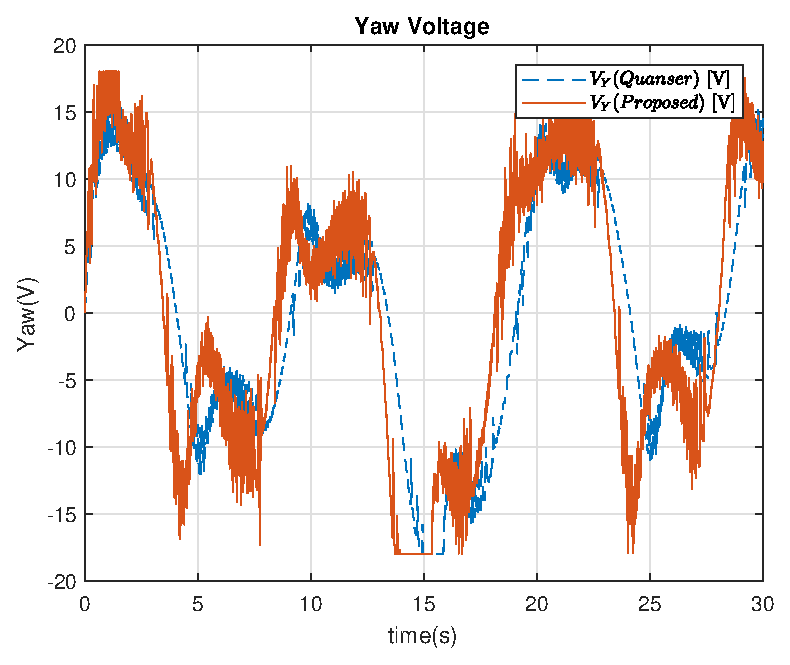
\includegraphics[width=.46\textwidth,keepaspectratio=true]{figs/matlab/LQR_PIvLQR_P_USB/sine/YawVoltage_LQR_RMSE.eps}
    \label{fig:YawVoltage_LQR_RMSE_Sine}
    }
    \subfigure[][]{
    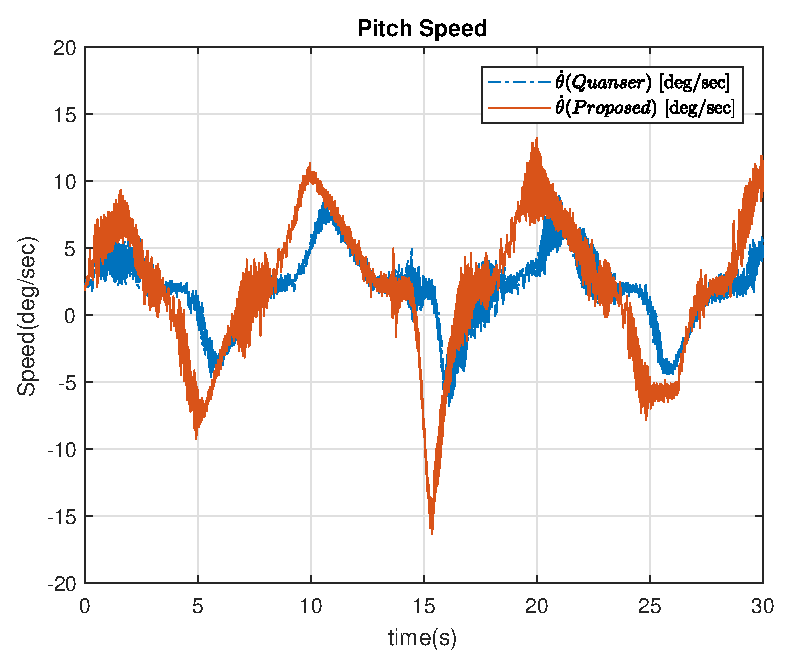
\includegraphics[width=.46\textwidth,keepaspectratio=true]{figs/matlab/LQR_PIvLQR_P_USB/sine/PitchSpeed_LQR_RMSE.eps}
    \label{fig:PitchSpeed_LQR_RMSE_Sine}
    }
    \subfigure[][]{
    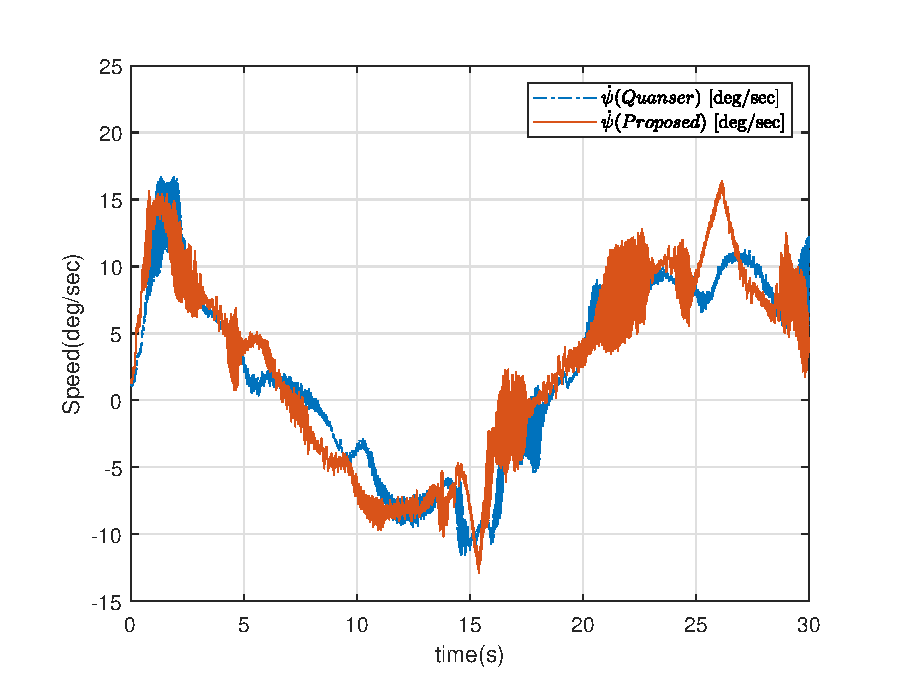
\includegraphics[width=.46\textwidth,keepaspectratio=true]{figs/matlab/LQR_PIvLQR_P_USB/sine/YawSpeed_LQR_RMSE.eps}
    \label{fig:PitchSpeed_LQR_RMSE_Sine}
    }
    \caption{USB implementation for proportional controller and proportional-integral controller calculated by LQR with a sinusoidal input.}
    \label{fig:PvsPI_Sine}
\end{figure}
%%----------------------------------------------------------------------
%\subsection{LQG (PI Controller)}
%%----------------------------------------------------------------------
%\todo[inline]{Insert LQG PI Block Diagram}
%\todo[inline]{Insert LQG PI Results}
%%----------------------------------------------------------------------
\subsection{ADP}
%----------------------------------------------------------------------
Figure~\ref{fig:ADP_P_USB_Block_Diagram} is the simulink model for the ADP motion control algorithm using the USB connection between the Quanser Aero and the PC.  It takes the desired configurations as the inputs and applies them and the actual states to the ADP block to calculate the voltages for the main and tail motors.  These are then applied directly to the helicopter trough the USB connection.
\begin{figure}[!htbp]
    \centering
    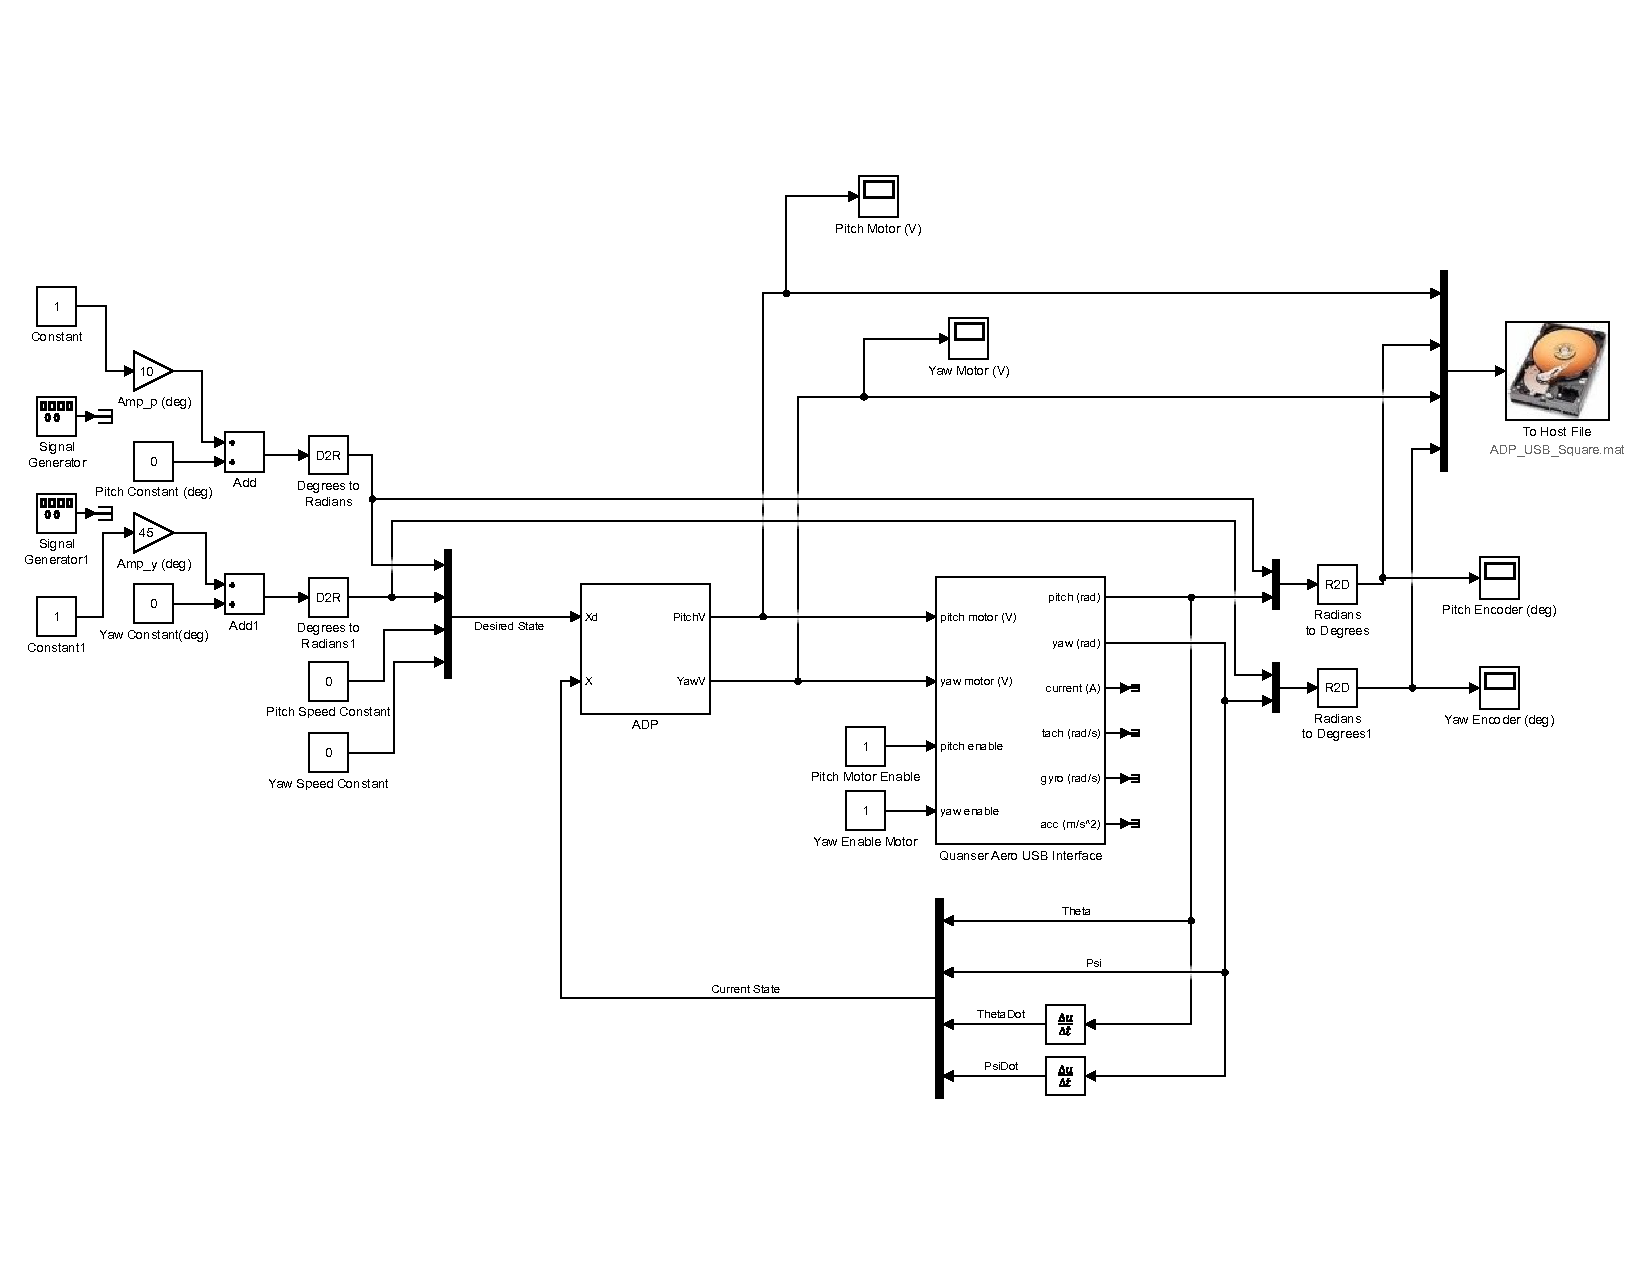
\includegraphics[width=.8\textwidth,keepaspectratio=true]{figs/img/ADP_USB}
    \caption{Block diagram for ADP P type controller with a USB connection.}
    \label{fig:ADP_P_USB_Block_Diagram}
\end{figure}
Figure~\ref{fig:ADP_P_BlackBox} is what is inside the ADP block in Figure~\ref{fig:ADP_P_USB_Block_Diagram}.
\begin{figure}[!htbp]
    \centering
    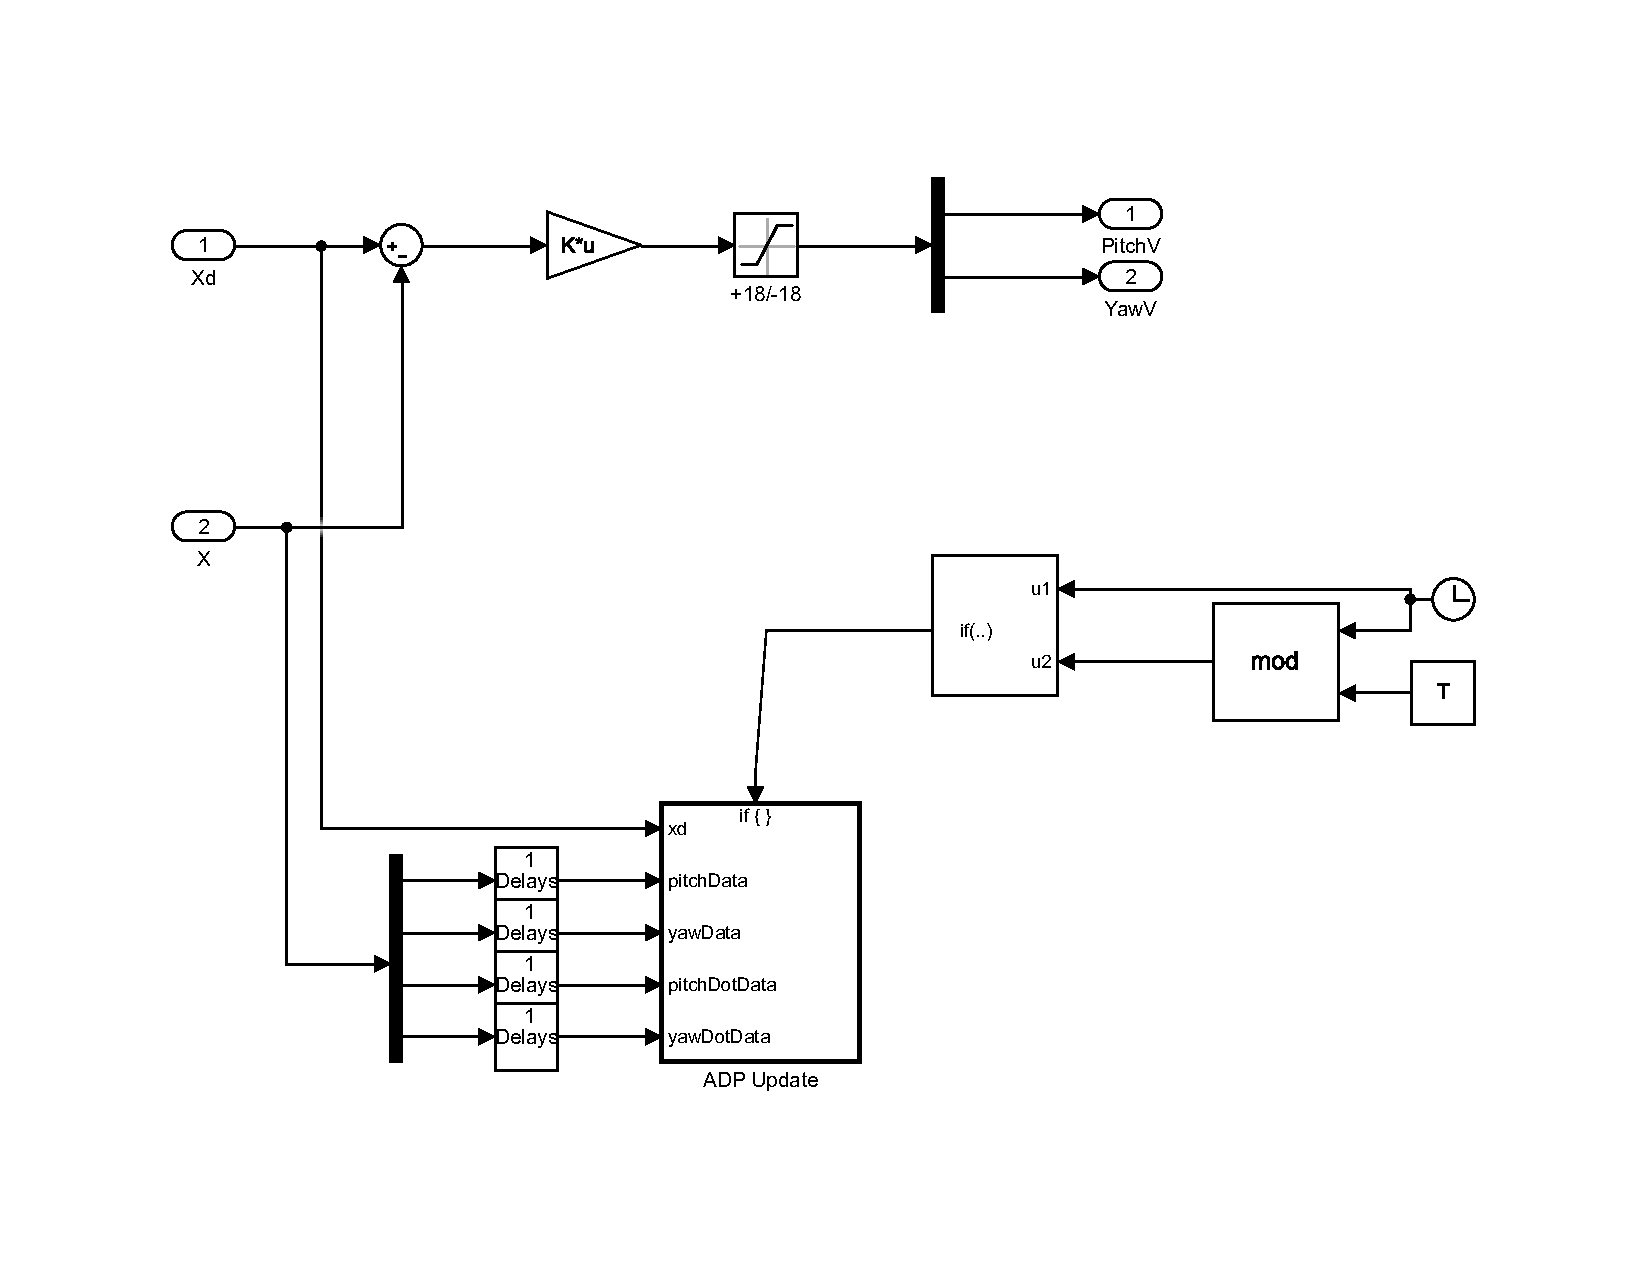
\includegraphics[width=.8\textwidth,keepaspectratio=true]{figs/img/ADP_Black_Box}
    \caption{Block diagram for ADP P type controller algorithm.}
    \label{fig:ADP_P_BlackBox}
\end{figure}

For the results of this experiment figure~\ref{fig:ADP_USB_Step} shows the results for ADP using a step input and USB connection.  Figure~\ref{fig:Pitch_ADP_RMSE_Step} shows the pitch configurations of both the actual and desired angles verses time.  Figure~\ref{fig:Yaw_ADP_RMSE_Step} shows the yaw configurations of both the actual and desired angles verses time.  Figure~\ref{fig:PitchVoltage_ADP_RMSE_Step} displays the voltage that is applied to the main motor verses time.  Figure~\ref{fig:YawVoltage_ADP_RMSE_Step} displays the voltage that is applied to the tail motor verses time.  Figure~\ref{fig:ADP_USB_Square} and figure~\ref{fig:ADP_USB_Sine} have similar figures to figure~\ref{fig:ADP_USB_Step}, except figure~\ref{fig:ADP_USB_Square} has a square wave input and figure~\ref{fig:ADP_USB_Sine} has a sine wave input.
\begin{figure}[!htbp]
    \centering
    \subfigure[][]{
    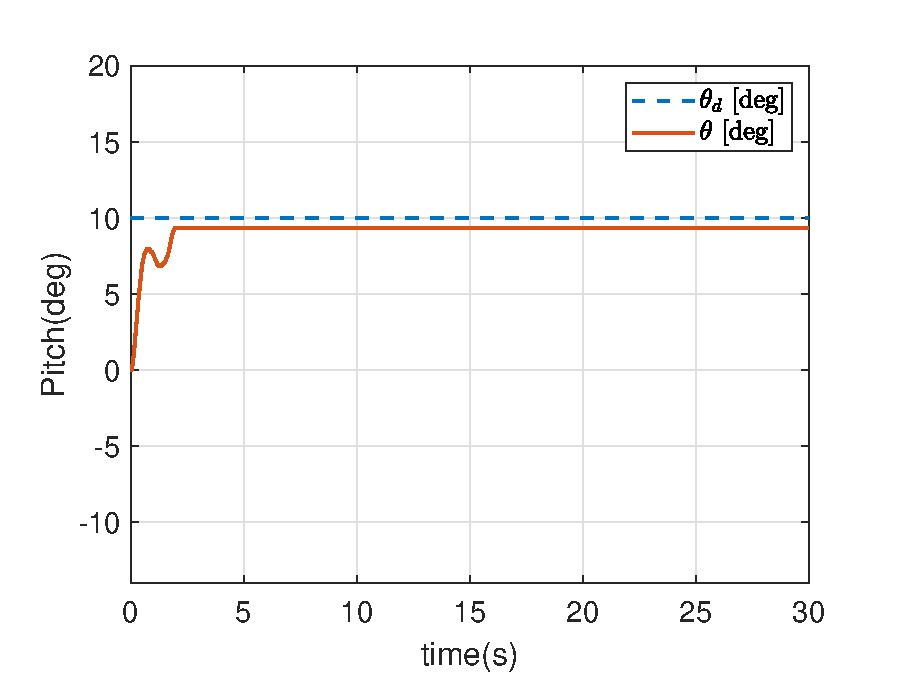
\includegraphics[width=.46\textwidth,keepaspectratio=true]{figs/matlab/ADP/USB/Pitch_ADP_Constant.eps}
    \label{fig:Pitch_ADP_RMSE_Step}
    }
    \subfigure[][]{
    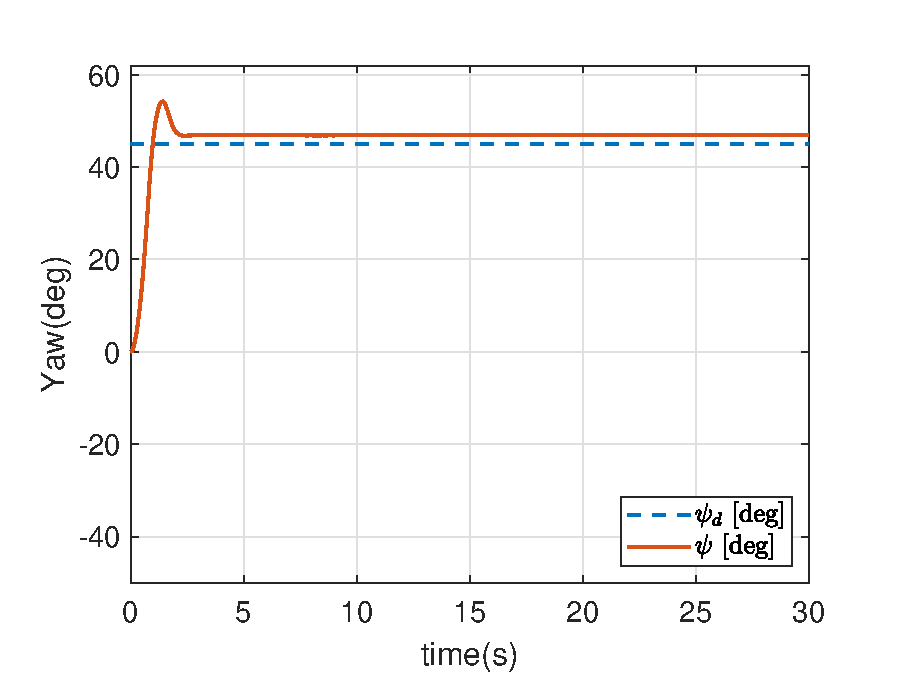
\includegraphics[width=.46\textwidth,keepaspectratio=true]{figs/matlab/ADP/USB/Yaw_ADP_Constant.eps}
    \label{fig:Yaw_ADP_RMSE_Step}
    }    
    \subfigure[][]{
    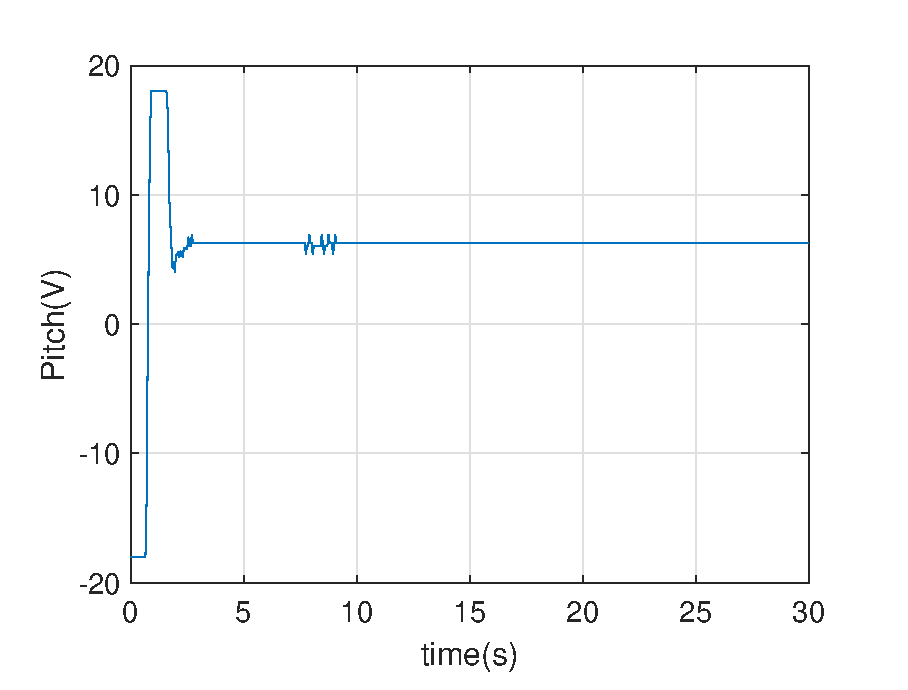
\includegraphics[width=.46\textwidth,keepaspectratio=true]{figs/matlab/ADP/USB/PitchVoltage_ADP_Constant.eps}
    \label{fig:PitchVoltage_ADP_RMSE_Step}
    }    
    \subfigure[][]{
    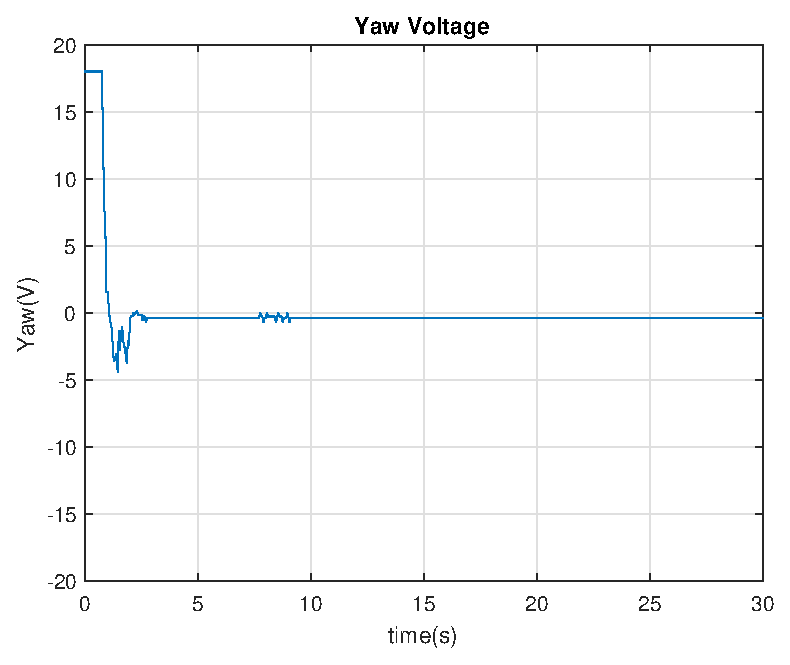
\includegraphics[width=.46\textwidth,keepaspectratio=true]{figs/matlab/ADP/USB/YawVoltage_ADP_Constant.eps}
    \label{fig:YawVoltage_ADP_RMSE_Step}
    }
    \caption{USB implementation for ADP proportional controller with a step input.}
    \label{fig:ADP_USB_Step}
\end{figure}

\begin{figure}[!htbp]
    \centering
    \subfigure[][]{
    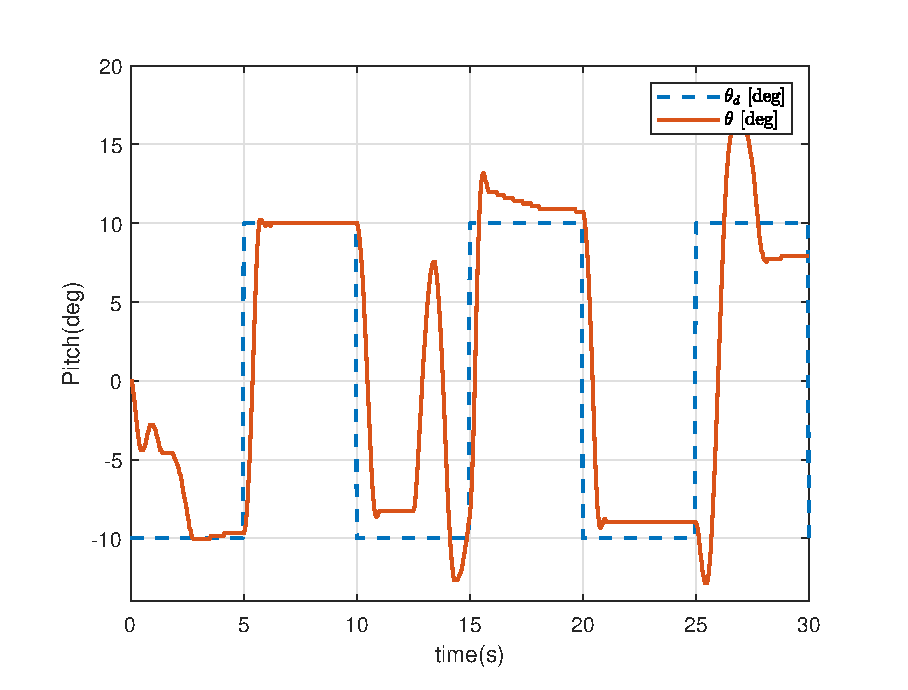
\includegraphics[width=.46\textwidth,keepaspectratio=true]{figs/matlab/ADP/USB/Pitch_ADP_Square.eps}
    \label{fig:Pitch_ADP_RMSE_Square}
    }
    \subfigure[][]{
    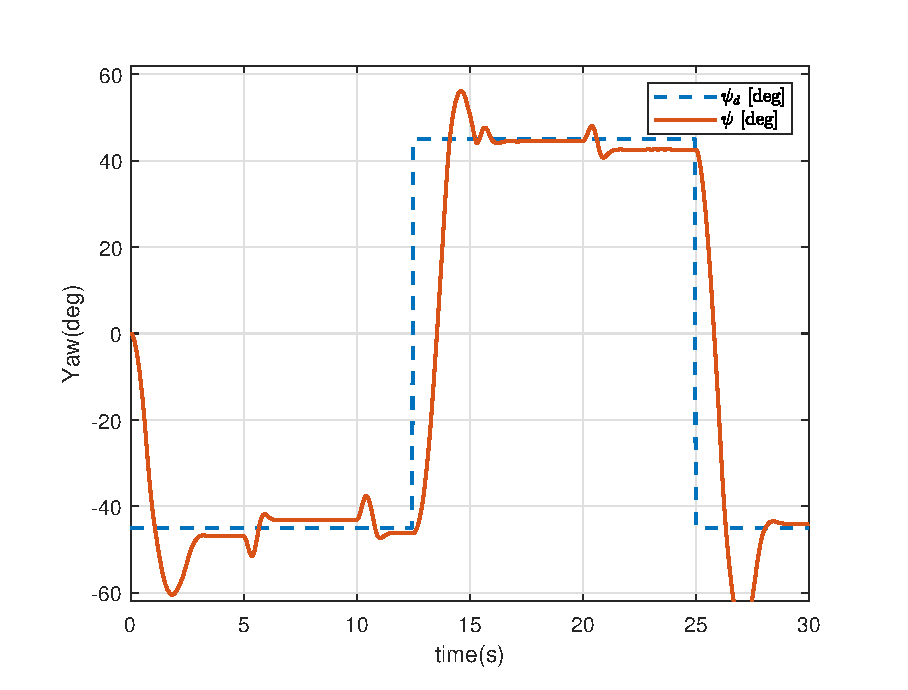
\includegraphics[width=.46\textwidth,keepaspectratio=true]{figs/matlab/ADP/USB/Yaw_ADP_Square.eps}
    \label{fig:Yaw_ADP_RMSE_Square}
    }    
    \subfigure[][]{
    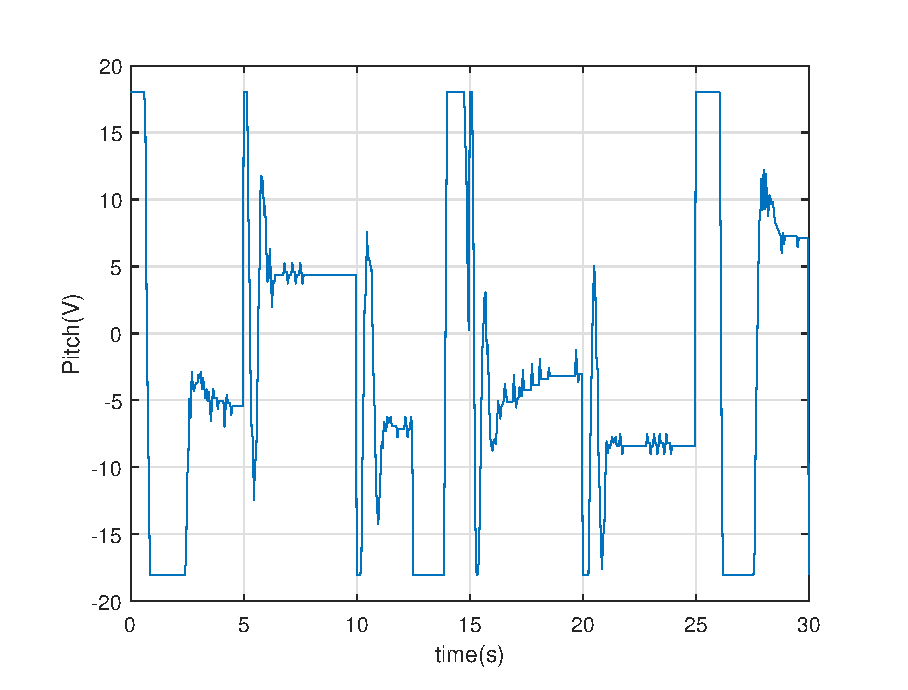
\includegraphics[width=.46\textwidth,keepaspectratio=true]{figs/matlab/ADP/USB/PitchVoltage_ADP_Square.eps}
    \label{fig:PitchVoltage_ADP_RMSE_Square}
    }    
    \subfigure[][]{
    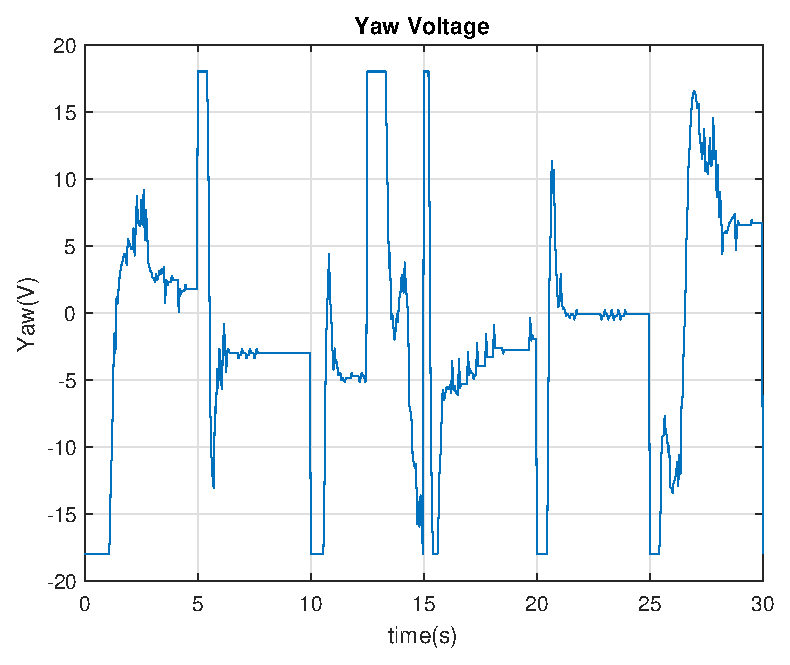
\includegraphics[width=.46\textwidth,keepaspectratio=true]{figs/matlab/ADP/USB/YawVoltage_ADP_Square.eps}
    \label{fig:YawVoltage_ADP_RMSE_Square}
    }
    \caption{USB implementation for ADP proportional controller with a square wave input.}
    \label{fig:ADP_USB_Square}
\end{figure}

\begin{figure}[!htbp]
    \centering
    \subfigure[][]{
    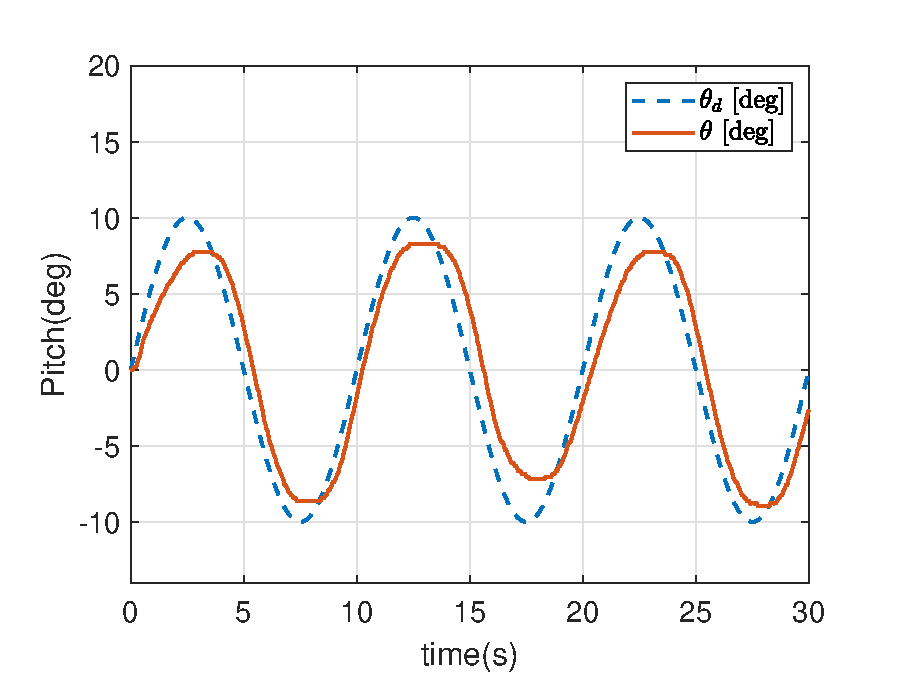
\includegraphics[width=.46\textwidth,keepaspectratio=true]{figs/matlab/ADP/USB/Pitch_ADP_Sine.eps}
    \label{fig:Pitch_ADP_RMSE_Sine}
    }
    \subfigure[][]{
    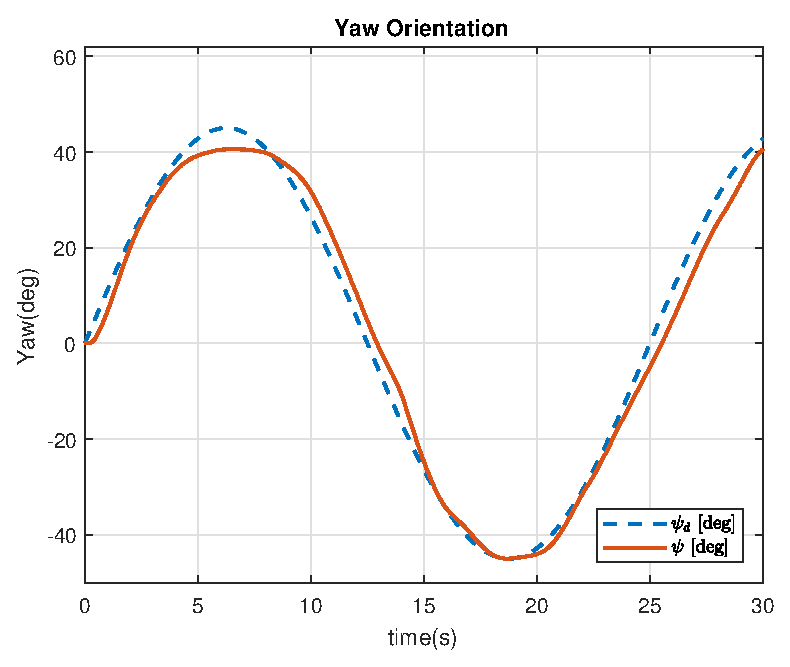
\includegraphics[width=.46\textwidth,keepaspectratio=true]{figs/matlab/ADP/USB/Yaw_ADP_Sine.eps}
    \label{fig:Yaw_ADP_RMSE_Sine}
    }    
    \subfigure[][]{
    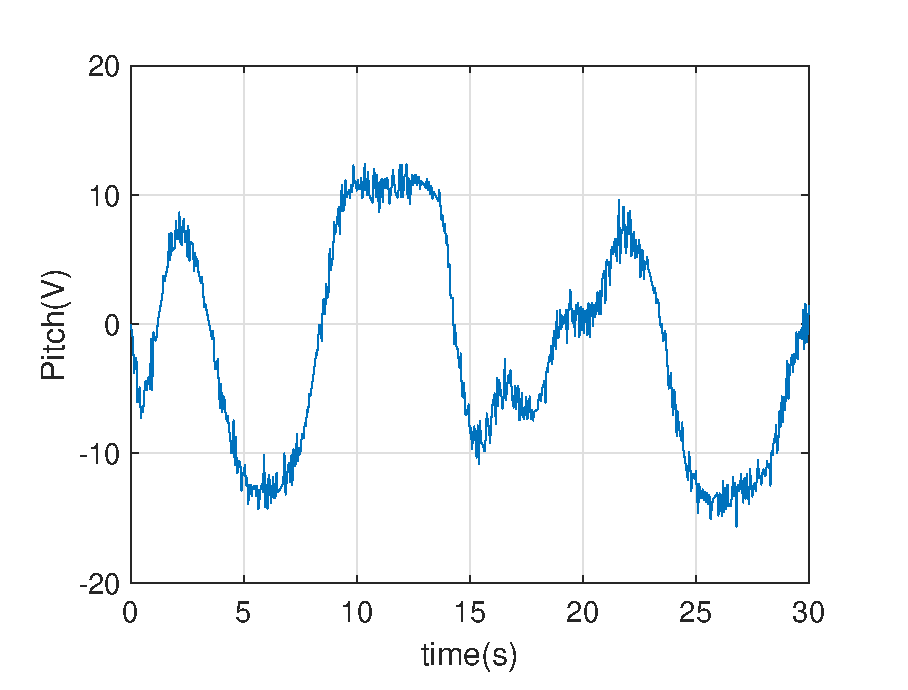
\includegraphics[width=.46\textwidth,keepaspectratio=true]{figs/matlab/ADP/USB/PitchVoltage_ADP_Sine.eps}
    \label{fig:PitchVoltage_ADP_RMSE_Sine}
    }    
    \subfigure[][]{
    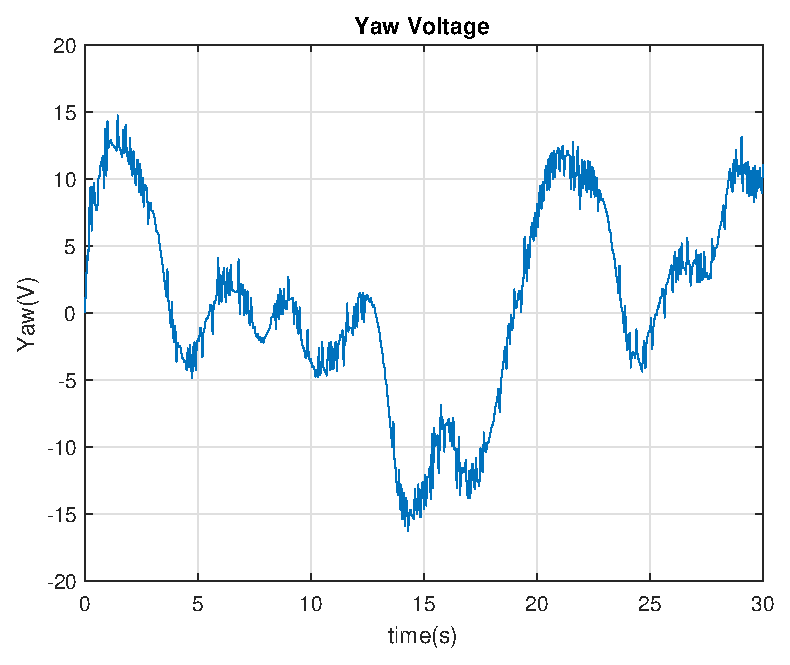
\includegraphics[width=.46\textwidth,keepaspectratio=true]{figs/matlab/ADP/USB/YawVoltage_ADP_Sine.eps}
    \label{fig:YawVoltage_ADP_RMSE_Sine}
    }
    \caption{USB implementation for ADP proportional controller with a sinusoidal input.}
    \label{fig:ADP_USB_Sine}
\end{figure}
%----------------------------------------------------------------------
\subsection{Root Mean Square Error}
%----------------------------------------------------------------------
Table~\ref{tab:RMSE_P_PI} give the root mean square error (RMSE) values for LQR P type verses LQR PI type controllers.  What the RMSE values show are the error distances to the desired configurations.  This table displays these values to show the improvement in the PI type controller compared to the P type controller.  Table~\ref{tab:RMSE_LQR_ADP} give the RMSE values for LQR P type verses ADP motion controllers.  This table displays these values to show the improvement in the ADP algorithm compared to the LQR P type controller algorithm.
%Note: constant used pitch 10 degrees, yaw 45 degrees\\
%Note: square used pitch XXXX degrees with period of XXXX, yaw XXXX degrees with period of XXXX\\
%Note: sine used pitch XXXX degrees with period of XXXX, yaw XXXX degrees with period of XXXX\\
%\begin{table}[h!]
%    \centering
%    \begin{tabular}{l|l|l|l|l|l|l}
%        \toprule
%        \textbf{} & \textbf{LQR(P)} & \textbf{LQR(PI)} &
%        \textbf{ADP(P)} \\
%        \toprule
%        RMSE Pitch Step & 2.6454 & ? & 1.3067 \\
%        RMSE Yaw Step & 5.7991 & ? & 6.1991 \\
%        RMSE Pitch Square & ? & ? & ? \\
%        RMSE Yaw Square & ? & ? & ? \\
%        RMSE Pitch Sine & ? & ? & ? \\
%        RMSE Yaw Sine & ? & ? & ? \\
%        \bottomrule
%    \end{tabular}
%    \caption{Error Comparison for USB Algorithms}
%    \label{tab:USB_RMSE}
%\end{table}
%Based on the results XXXX preformed better for USB.

\begin{table}
    \centering
    \begin{tabular}{l|l|l|l|l|l|l}
        \toprule
        \textbf{} & \textbf{Pitch Step} & \textbf{Yaw Step} & \textbf{Pitch Squ.} & \textbf{Yaw Squ.} & \textbf{Pitch Sine} & \textbf{Yaw Sine}\\
        \toprule
        LQR P & 3.5025 & 5.8502 & 6.2819 & 20.4623 & 4.2469 & 2.8644\\
        LQR PI & 1.2349 & 5.5058 & 6.9206 & 21.0709 & 1.3383 & 1.7852\\
        Improvement & 64.7437\% & 0.5408\% & -10.1675\% & -2.9740\% & 68.4872\% & 63.2998\% \\
    \end{tabular}
    \caption{Root mean squared error and improvement for LQR P and PI controller}
    \label{tab:RMSE_P_PI}
\end{table}

\begin{table}
    \centering
    \begin{tabular}{l|l|l|l|l|l|l}
        \toprule
        \textbf{} & \textbf{Pitch Step} & \textbf{Yaw Step} & \textbf{Pitch Squ.} & \textbf{Yaw Squ.} & \textbf{Pitch Sine} & \textbf{Yaw Sine}\\
        \toprule
        LQR P & 3.5025 & 5.8502 & 6.2819 & 20.4623 & 4.2469 & 2.8644\\
        ADP P & 1.3067 & 6.1991 & 6.5790 & 21.1923 & 2.1877 & 3.6307\\
        Improvement & 62.6923\% & -5.9638\%  & -4.7294\% & -0.3567\% & 48.4871\% & -26.7525\% \\
    \end{tabular}
    \caption{Root mean squared error and improvement for LQR P and ADP P controller}
    \label{tab:RMSE_LQR_ADP}
\end{table}
%----------------------------------------------------------------------

%======================================================================
\section{Raspberry Pi}
Before the algorithms were implemented using the mobile device they were tested using only the raspberry pi to make sure that the wireless communication worked.
%----------------------------------------------------------------------
\subsection{LQR (P Type Controller)}
%----------------------------------------------------------------------
Figure~\ref{fig:LQR_RaspPi} shows the simulink model that was built to the raspberry pi to test the LQR P type algorithm.  It can be seen that it takes predetermined constant inputs to set the desired configuration.  Those desired values are subtracted by the actual state which is then multiplied by the control gain and sent to the Quanser Aero via the SPI connection with the raspberry pi.
\begin{figure}[!htbp]
    \centering
    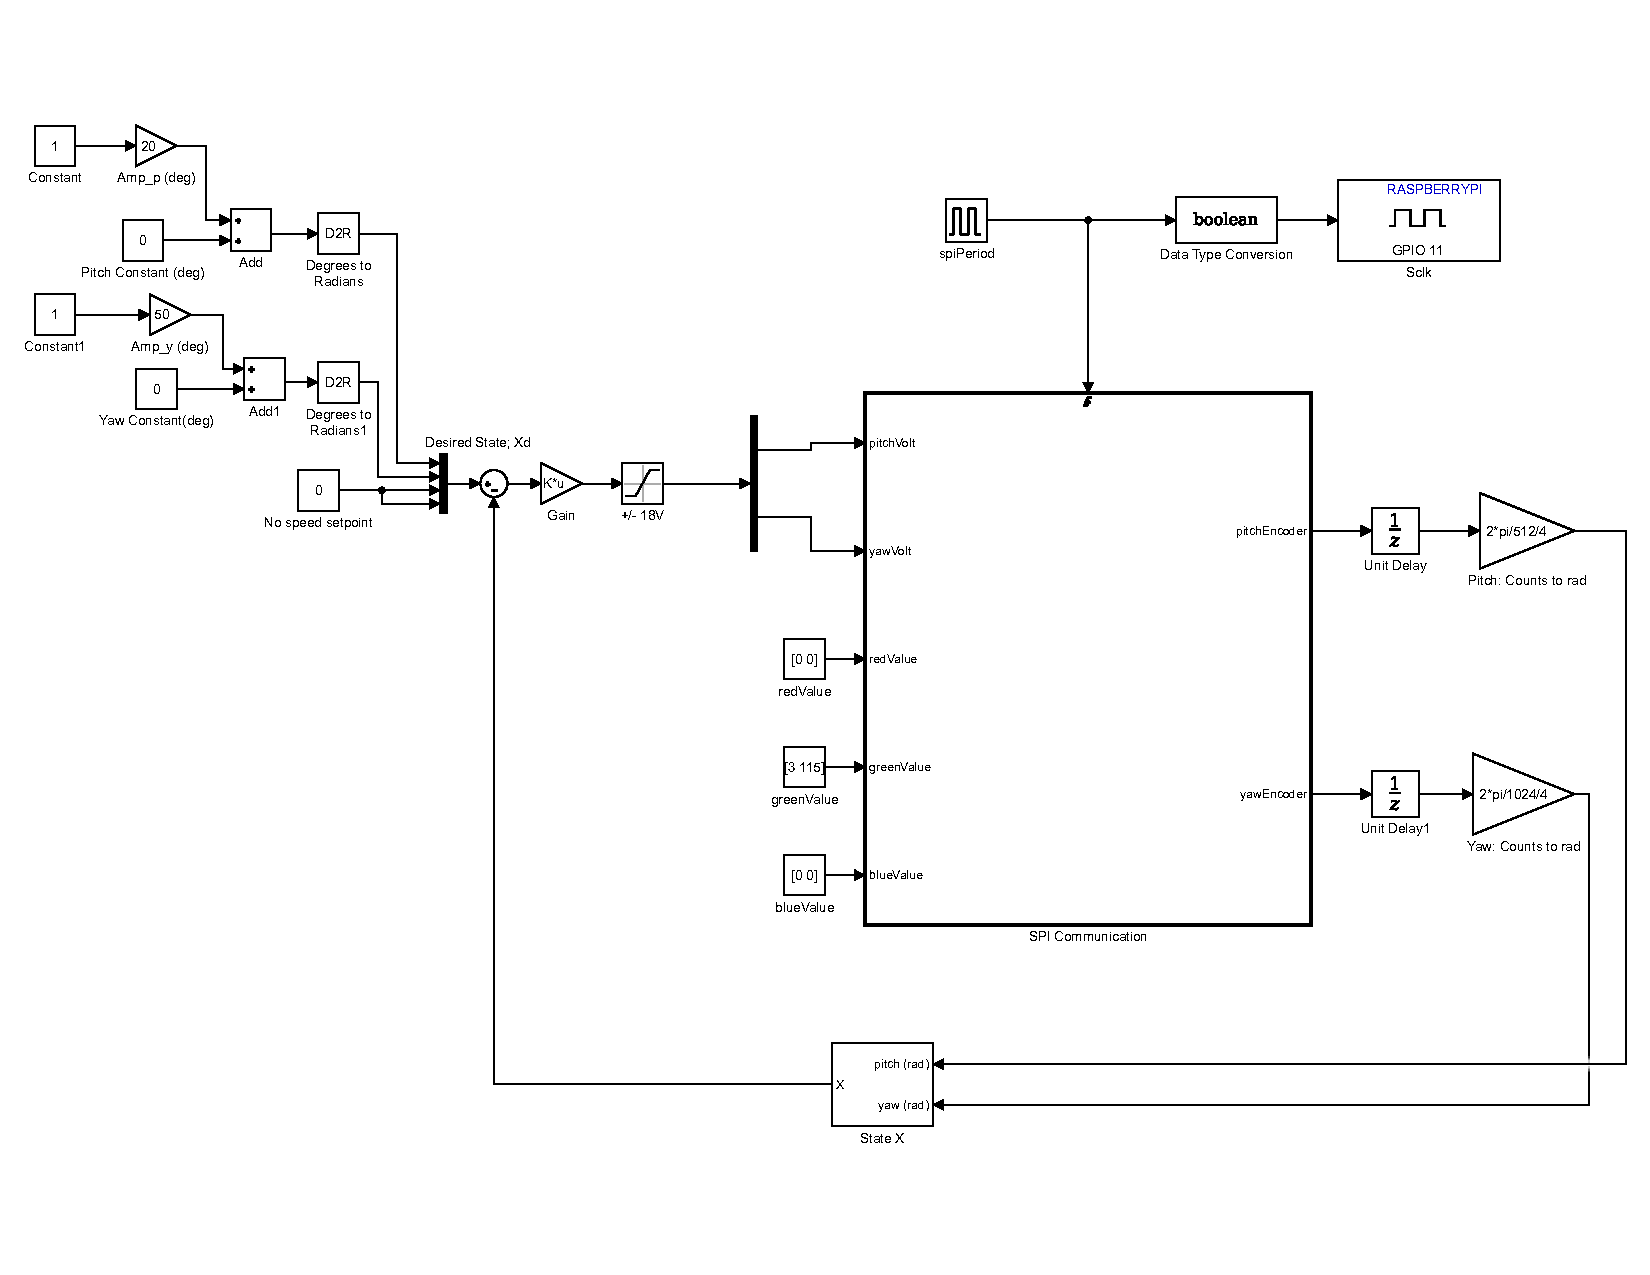
\includegraphics[width=.62\textwidth,keepaspectratio=true]{figs/img/LQR_RaspPi}
    \caption{Simulink model of LQR P type using raspberry pi communication.}
    \label{fig:LQR_RaspPi}
\end{figure}


%----------------------------------------------------------------------
\subsection{ADP}
%----------------------------------------------------------------------
Figure~\ref{fig:ADP_RaspPi} shows the simulink model that was built to the raspberry pi to test the ADP algorithm.  It can be seen that it takes predetermined constant inputs to set the desired configuration.  Those desired values as well as the actual configuration values are sent into the ADP block which calculates the voltages to be applied to the system.  These voltages are then sent to the Quanser Aero via the SPI connection with the raspberry pi.
\begin{figure}[!htbp]
    \centering
    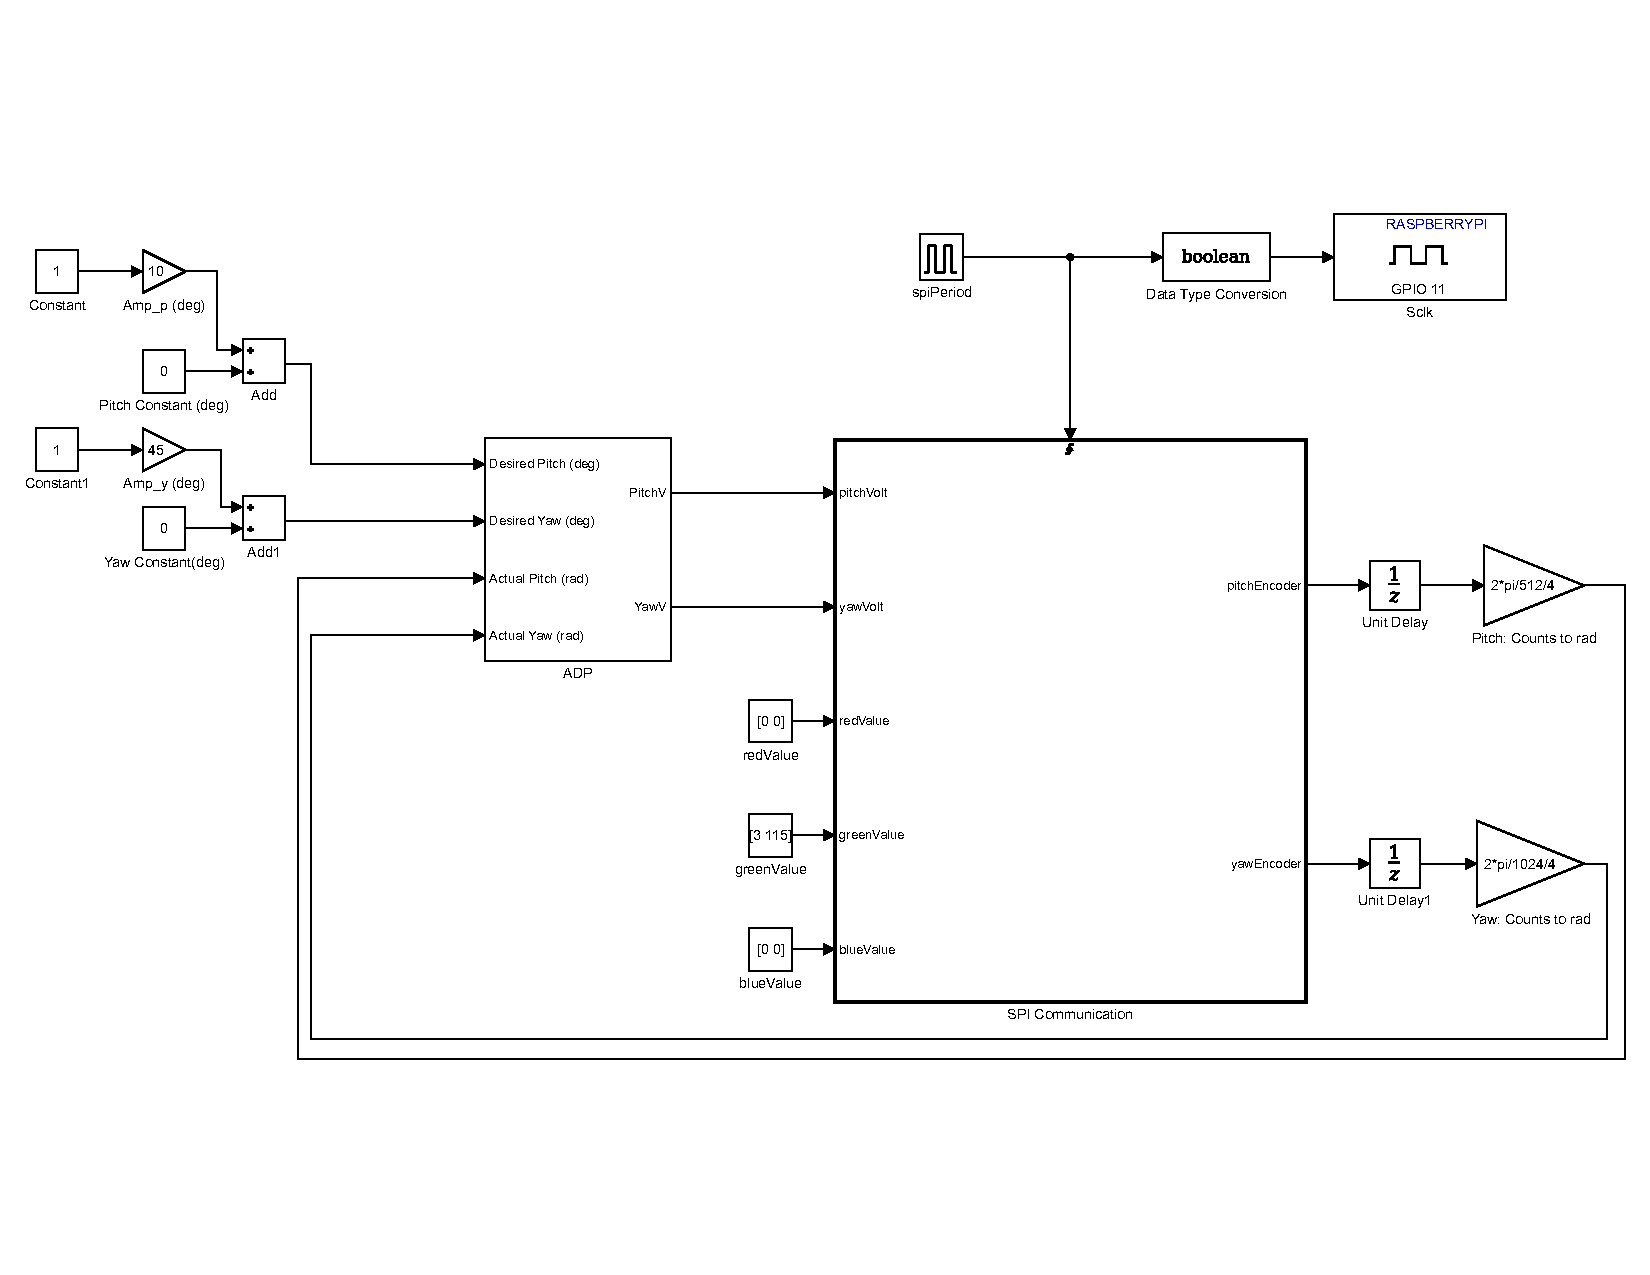
\includegraphics[width=.62\textwidth,keepaspectratio=true]{figs/img/ADP_RaspPi}
    \caption{Simulink model of ADP using raspberry pi communication.}
    \label{fig:ADP_RaspPi}
\end{figure}
%\todo[inline]{Insert ADP P Results}

%%----------------------------------------------------------------------
%\subsection{Conclusions}
%%----------------------------------------------------------------------
%Note: constant used pitch XXXX degrees, yaw XXXX degrees\\
%Note: square used pitch XXXX degrees with period of XXXX, yaw XXXX degrees with period of XXXX\\
%Note: sine used pitch XXXX degrees with period of XXXX, yaw XXXX degrees with period of XXXX\\
%\begin{table}[h!]
%    \centering
%    \begin{tabular}{l|l|l|l|l|l|l}
%        \toprule
%        \textbf{} & \textbf{LQR(P)} & \textbf{ADP(P)} \\
%        \toprule
%        RMSE Pitch Step & ? & ?  \\
%        RMSE Yaw Step & ? & ? \\
%        RMSE Pitch Square & ? & ? \\
%        RMSE Yaw Square & ? & ? \\
%        RMSE Pitch Sine & ? & ? \\
%        RMSE Yaw Sine & ? & ? \\
%        \bottomrule
%    \end{tabular}
%    \caption{Error Comparison for USB Algorithms}
%    \label{tab:USB_RMSE}
%\end{table}
%Based on the results XXXX preformed better for Raspberry Pi.
%----------------------------------------------------------------------

%======================================================================
\section{Mobile Device}
Testing and implementation using the mobile device user interface was then done for the LQR p type and ADP motion control algorithms.
%----------------------------------------------------------------------
\subsection{LQR (P Type Controller)}
%----------------------------------------------------------------------
Figure~\ref{fig:LQR_Android} is the simulink model for mobile device communication using LQR p type motion control algoritm.  As it can be seen the desired configurations are taken in from the mobile device using UDP receive blocks.  These values are then sent into the LQR block with the actual configurations to calculate the voltages for the two motors.  These voltage values are then sent to the Quanser Aero from the raspberry pi using the SPI communication.  The actual configuration values are then read from the Quanser Aero using the SPI communication, then the raspberry pi sends those actual configuration values to the mobile device using UDP send blocks.
\begin{figure}[!htbp]
    \centering
    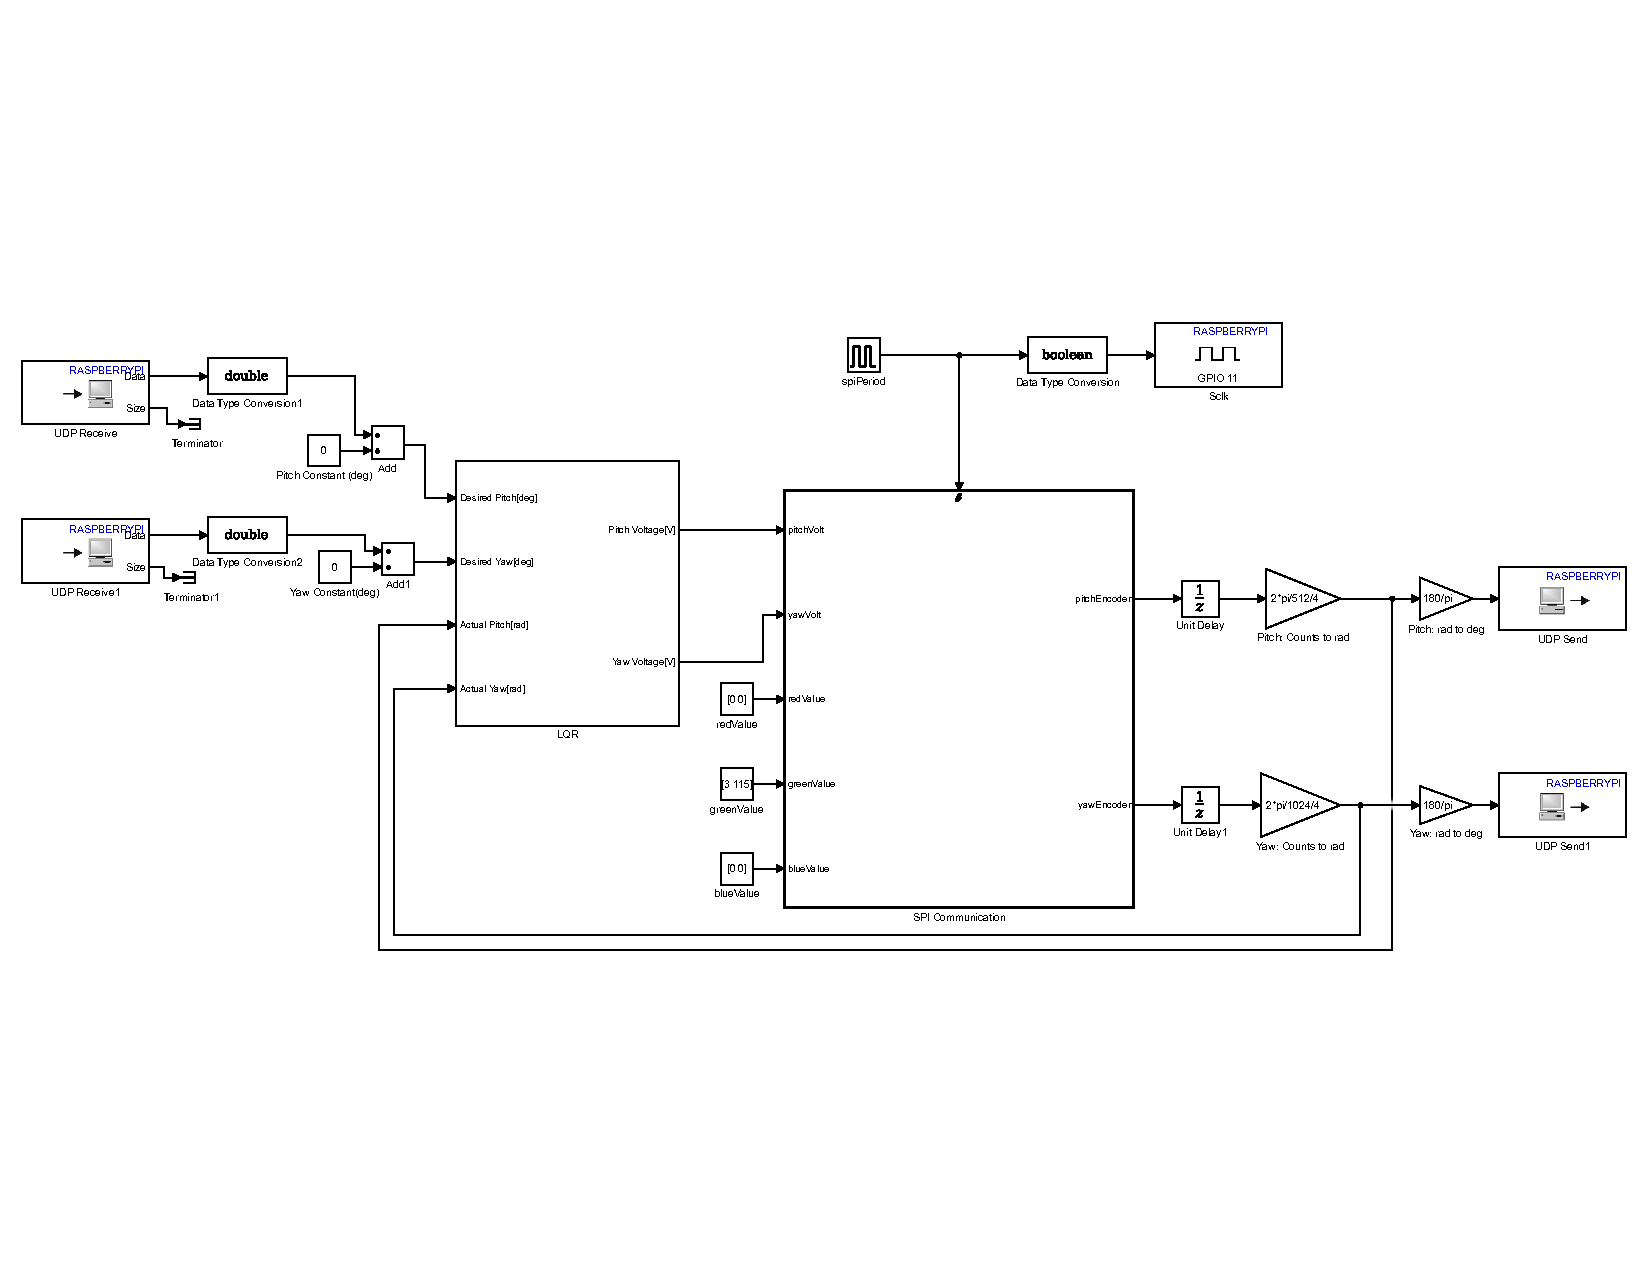
\includegraphics[width=.72\textwidth,keepaspectratio=true]{figs/img/LQR_Android}
    \caption{Simulink model of LQR using mobile device communication.}
    \label{fig:LQR_Android}
\end{figure}

The figure~\ref{fig:AndroidLQR} shows the results of the implementation using LQR p type for the mobile device user interface.  Figure~\ref{fig:AndroidLQRPitchpos} shows the actual pitch configuration and the desired that was set using the mobile device verses time.  Figure~\ref{fig:AndroidLQRYawpos} shows the actual yaw configuration and the desired that was set using the mobile device verses time.  As can be seen, the actual configuration tries to follow the wave form that is being set by the user.  Figure~\ref{fig:AndroidLQRPitchVolt} and figure~\ref{fig:AndroidLQRPitchVolt} show the voltages that are applied to the main and tail motors to get these motions in the pitch and yaw directions.
\begin{figure}
    \centering
    \subfigure[][]{
    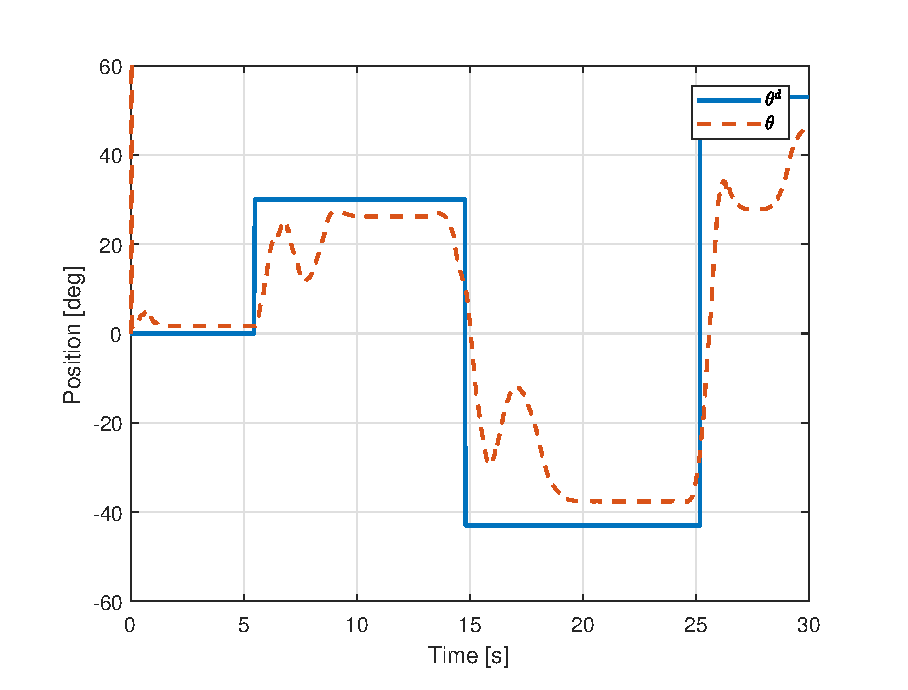
\includegraphics[width=.46\textwidth,keepaspectratio=true]{figs/matlab/LQR/P_Android/LQR_Pitchpos.eps}
    \label{fig:AndroidLQRPitchpos}
    }
    \subfigure[][]{
    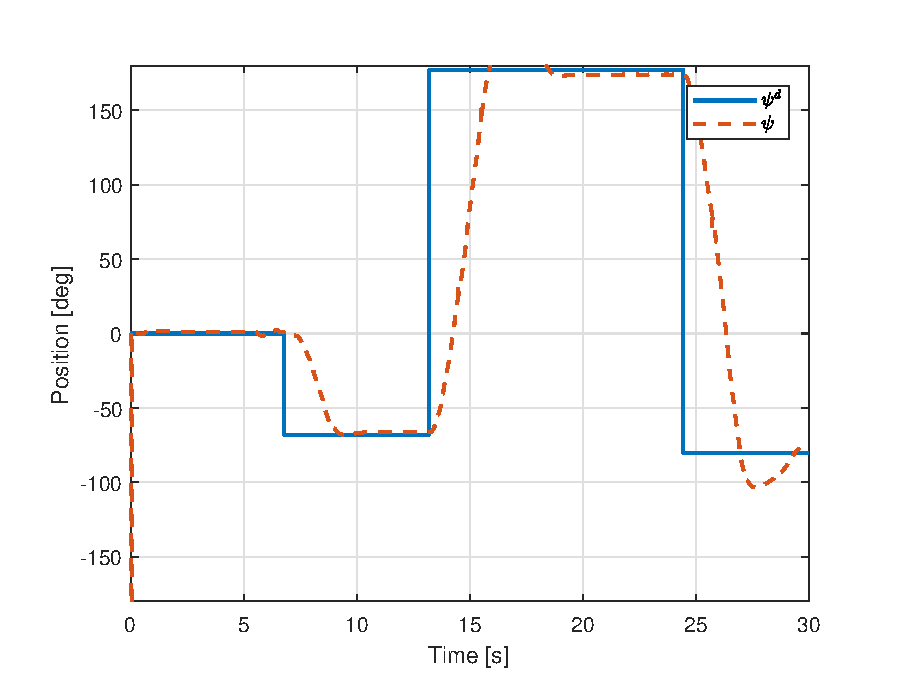
\includegraphics[width=.46\textwidth,keepaspectratio=true]{figs/matlab/LQR/P_Android/LQR_Yawpos.eps}
    \label{fig:AndroidLQRYawpos}
    }
    \subfigure[][]{
    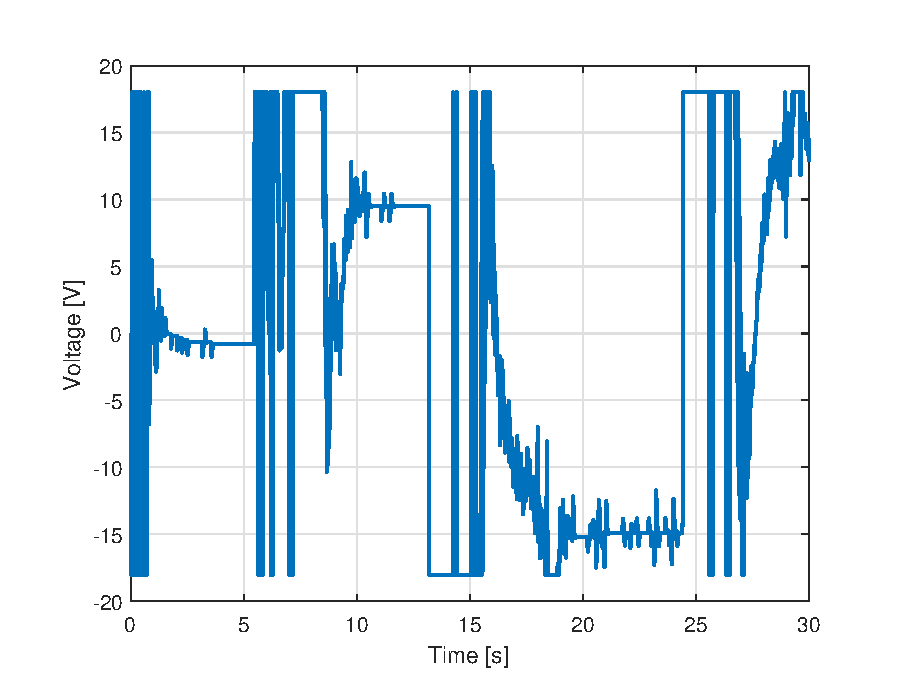
\includegraphics[width=.46\textwidth,keepaspectratio=true]{figs/matlab/LQR/P_Android/LQR_PitchVolt.eps}
    \label{fig:AndroidLQRPitchVolt}
    }
    \subfigure[][]{
    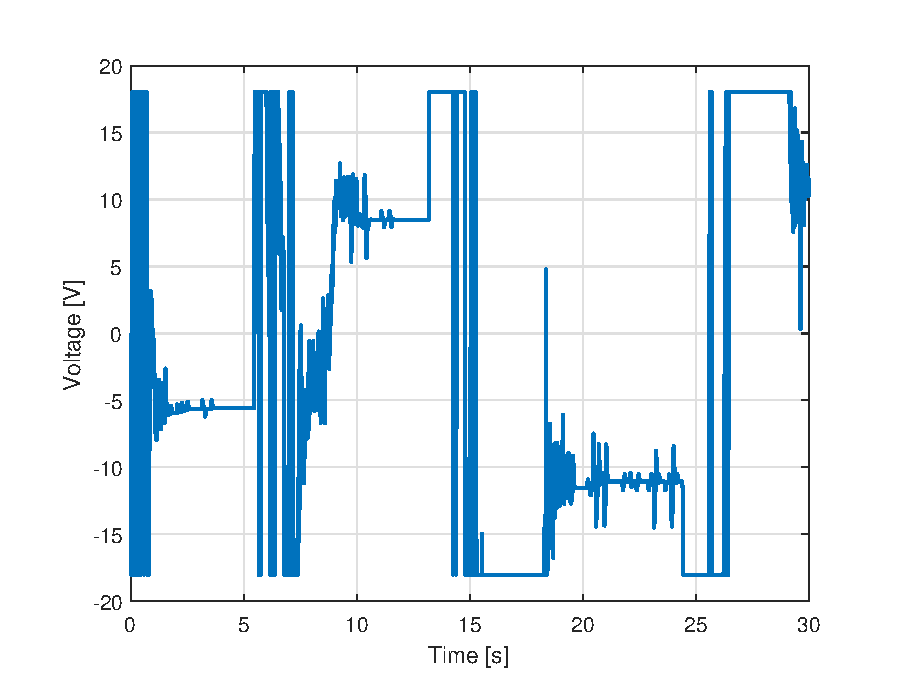
\includegraphics[width=.46\textwidth,keepaspectratio=true]{figs/matlab/LQR/P_Android/LQR_YawVolt.eps}
    \label{fig:AndroidLQRYawVolt}
    }
    \caption{Implementation results for LQR P type controller using mobile device as user input.}
    \label{fig:AndroidLQR}
\end{figure}


%----------------------------------------------------------------------
\subsection{ADP}
%----------------------------------------------------------------------
Figure~\ref{fig:ADP_Android} is the simulink model for mobile device communication using the ADP motion control algoritm.  As it can be seen the desired configurations are taken in from the mobile device using UDP receive blocks.  These values are then sent into the ADP block with the actual configurations to calculate the voltages for the two motors.  These voltage values are then sent to the Quanser Aero from the raspberry pi using the SPI communication.  The actual configuration values are then read from the Quanser Aero using the SPI communication, then the raspberry pi sends those actual configuration values to the mobile device using UDP send blocks.
\begin{figure}[!htbp]
    \centering
    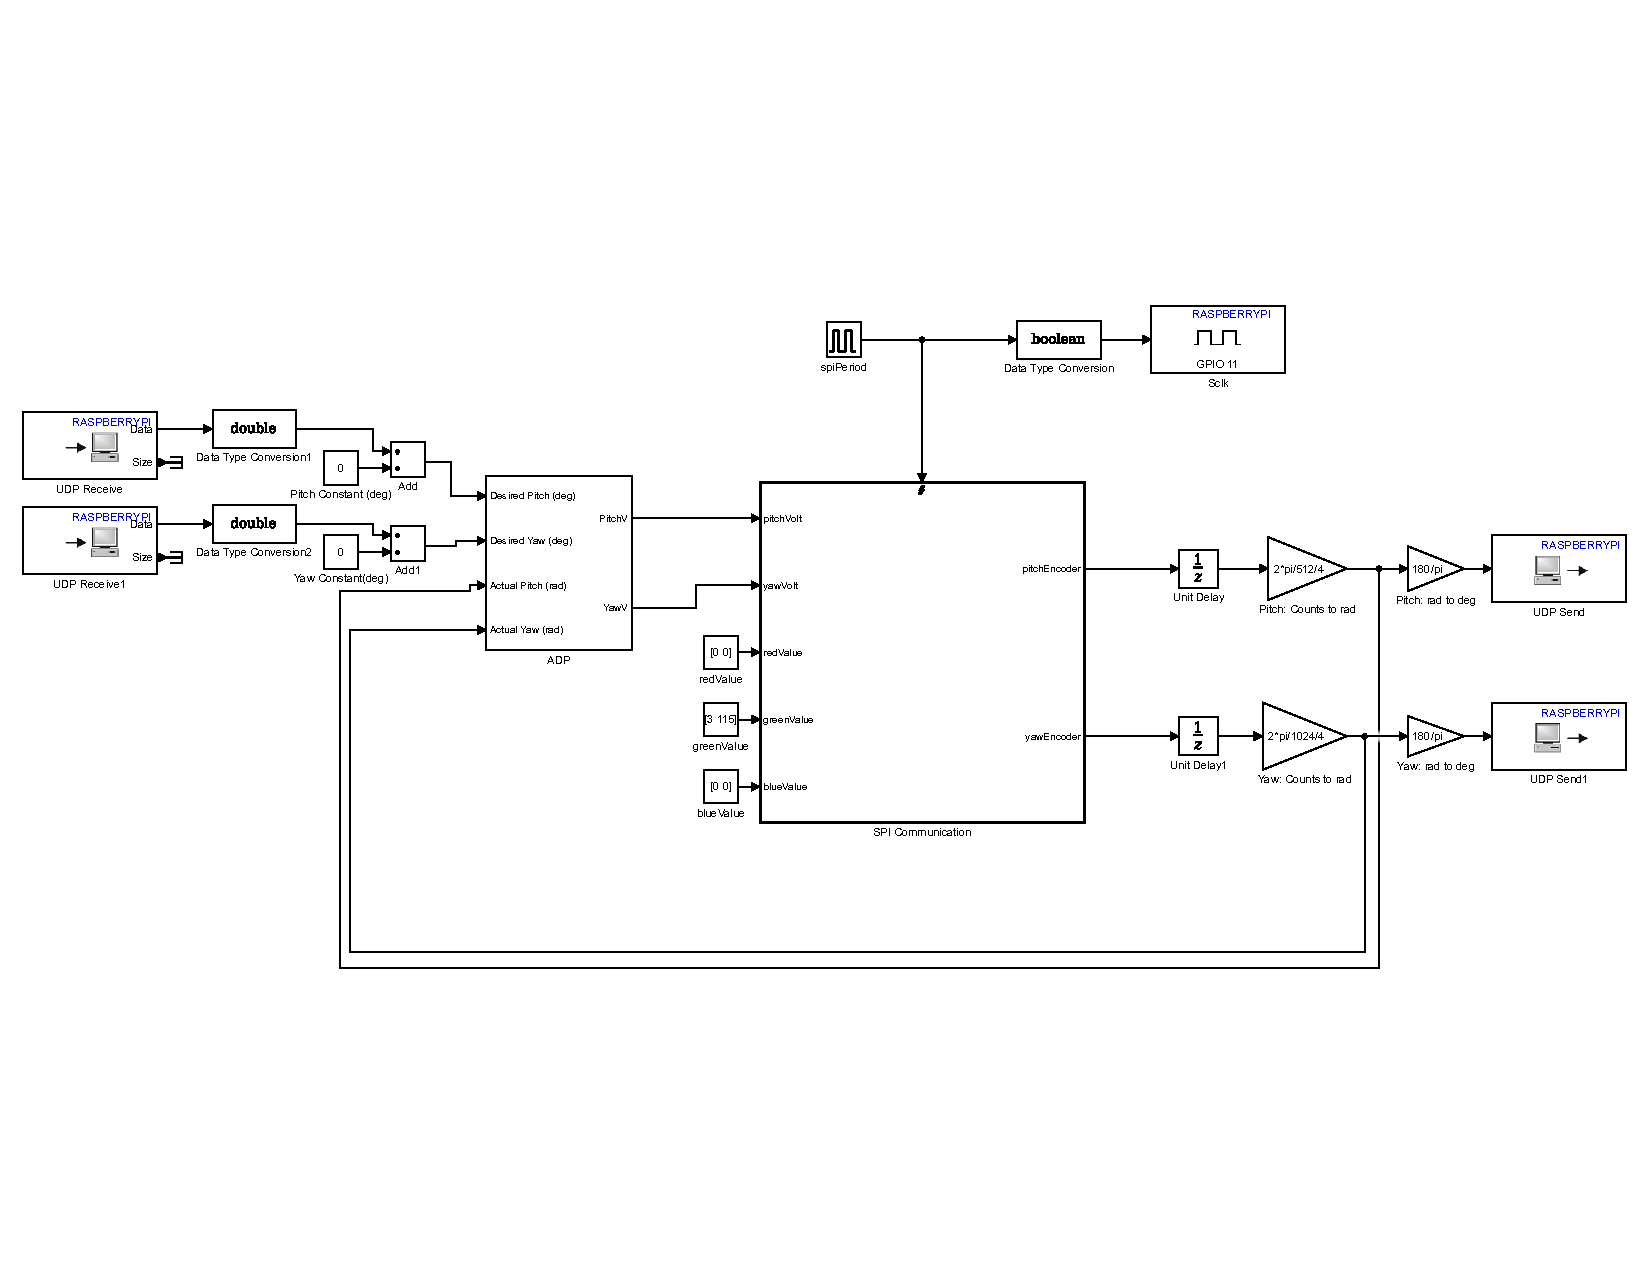
\includegraphics[width=.72\textwidth,keepaspectratio=true]{figs/img/ADP_Android}
    \caption{Simulink model of ADP using mobile device communication.}
    \label{fig:ADP_Android}
\end{figure}

The figure~\ref{fig:AndroidADP} shows the results of the implementation using ADP for the mobile device user interface.  Figure~\ref{fig:AndroidADPPitchpos} shows the actual pitch configuration and the desired that was set using the mobile device verses time.  Figure~\ref{fig:AndroidADPYawpos} shows the actual yaw configuration and the desired that was set using the mobile device verses time.  As can be seen, the actual configuration tries to follow the wave form that is being set by the user.  Figure~\ref{fig:AndroidADPPitchVolt} and figure~\ref{fig:AndroidADPPitchVolt} show the voltages that are applied to the main and tail motors to get these motions in the pitch and yaw directions.
\begin{figure}
    \centering
    \subfigure[][]{
    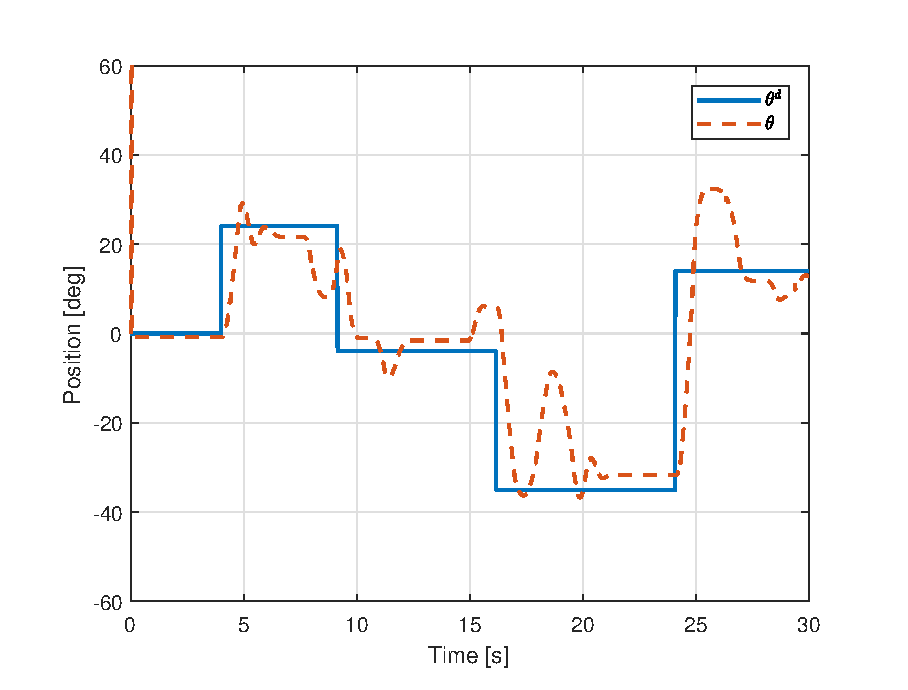
\includegraphics[width=.46\textwidth,keepaspectratio=true]{figs/matlab/ADP/Android/ADP_Pitch_Wireless.eps}
    \label{fig:AndroidADPPitchpos}
    }
    \subfigure[][]{
    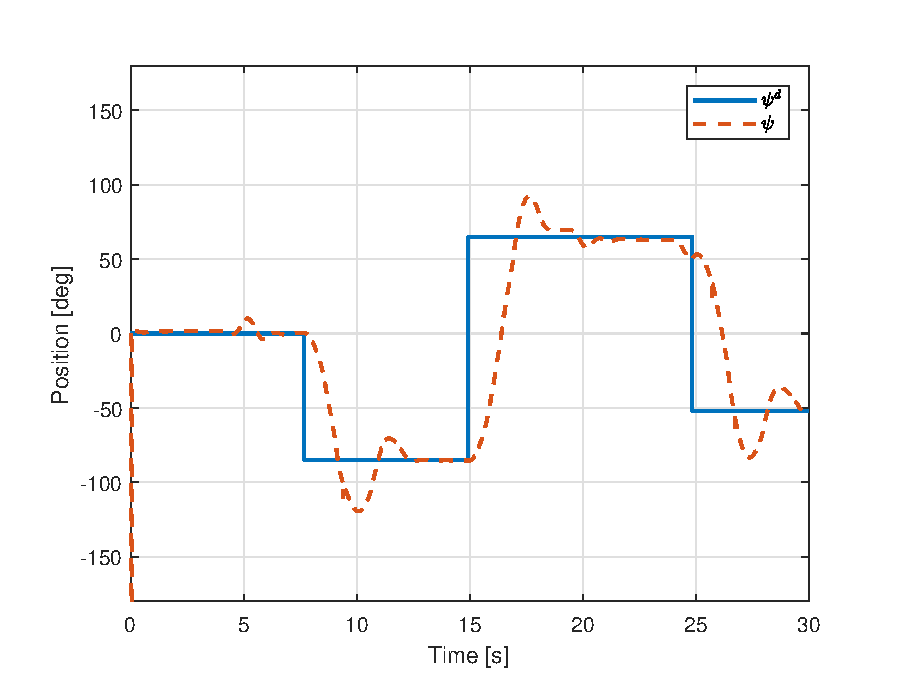
\includegraphics[width=.46\textwidth,keepaspectratio=true]{figs/matlab/ADP/Android/ADP_Yaw_Wireless.eps}
    \label{fig:AndroidADPYawpos}
    }
    \subfigure[][]{
    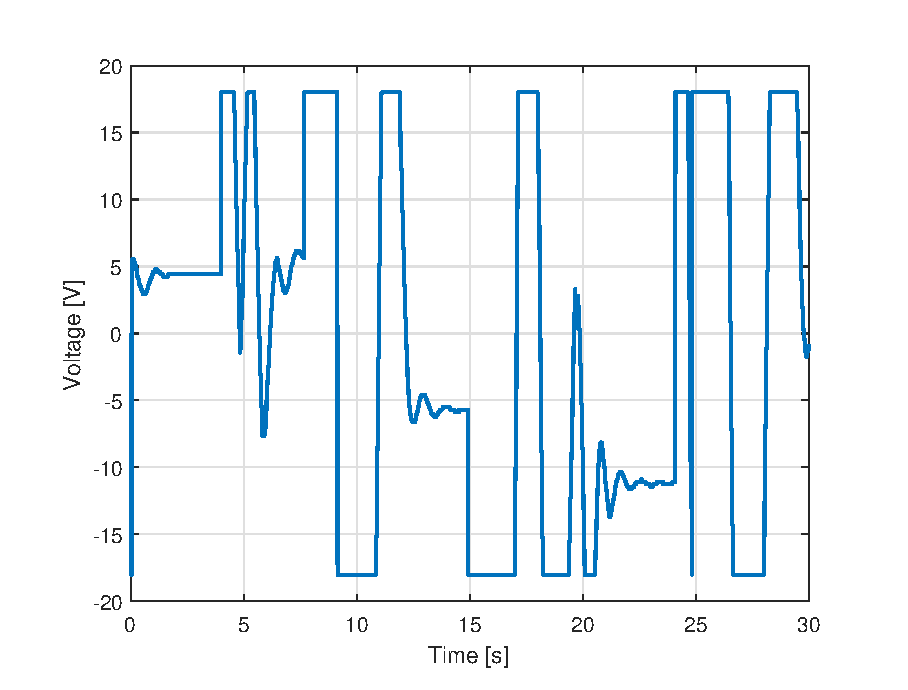
\includegraphics[width=.46\textwidth,keepaspectratio=true]{figs/matlab/ADP/Android/ADP_Pitch_Volt_Wireless.eps}
    \label{fig:AndroidADPPitchVolt}
    }
    \subfigure[][]{
    \includegraphics[width=.46\textwidth,keepaspectratio=true]{figs/matlab/ADP/Android/ADP_Yaw_Volt_Wireless.eps}
    \label{fig:AndroidADPYawVolt}
    }
    \caption{Implementation results for ADP controller using mobile device as user input.}
    \label{fig:AndroidADP}
\end{figure}

%%----------------------------------------------------------------------
%\subsection{Conclusions}
%%----------------------------------------------------------------------
%Note: constant used pitch XXXX degrees, yaw XXXX degrees\\
%Note: square used pitch XXXX degrees with period of XXXX, yaw XXXX degrees with period of XXXX\\
%Note: sine used pitch XXXX degrees with period of XXXX, yaw XXXX degrees with period of XXXX\\
%\begin{table}[h!]
%    \centering
%    \begin{tabular}{l|l|l|l|l|l|l}
%        \toprule
%        \textbf{} & \textbf{LQR(P)} & \textbf{ADP(P)} \\
%        \toprule
%        RMSE Pitch Step & ? & ?  \\
%        RMSE Yaw Step & ? & ? \\
%        RMSE Pitch Square & ? & ? \\
%        RMSE Yaw Square & ? & ? \\
%        RMSE Pitch Sine & ? & ? \\
%        RMSE Yaw Sine & ? & ? \\
%        \bottomrule
%    \end{tabular}
%    \caption{Error Comparison for USB Algorithms}
%    \label{tab:USB_RMSE}
%\end{table}
%Based on the results XXXX preformed better for Android.

%----------------------------------------------------------------------


%%% Local Variables:
%%% mode: latex
%%% TeX-master: "../finalReport"
%%% End:
